\documentclass{mooiman_memo}
\bibliography{c:/Users/janmo/checkouts/git/examples/references/literature_references.bib}

\usepackage{dutchcal}

\usepackage{bm}
\renewcommand{\vec}[1]{\mbox{\boldmath ${#1}$} }

\sisetup{mode=math}
\captionsetup[subfigure]{justification=RaggedRight}

\allowdisplaybreaks[1]

\newcommand{\ii}{{\rm i}}
\newcommand{\Dx}{\Delta x}
\newcommand{\Dy}{\Delta y}
\newcommand{\Dh}{\Delta h}
\newcommand{\Dq}{\Delta q}
\newcommand{\Dr}{\Delta r}
\newcommand{\Dxi}{\Delta \xi}
\newcommand{\Deta}{\Delta \eta}
\newcommand{\Dt}{\Delta t}
\newcommand{\Dtinv}{\Delta t_{\it{inv}}}
\newcommand{\Du}{\Delta u}
\newcommand{\vecn}{\mathbcal{n}}  % normal component in eta-direction
\newcommand{\nx}{\mathcal{n}_x}  % normal component in x-direction
\newcommand{\ny}{\mathcal{n}_y}  % normal component in y-direction
\newcommand{\nxi}{\mathcal{n}_\xi}  % normal component in xi-direction
\newcommand{\neta}{\mathcal{n}_\eta}  % normal component in eta-direction

\newcommand{\mat}[1]{\mbox{\boldmath ${\rm #1}$} }
\newcommand{\half}{\frac{1}{2}}
\newcommand{\quart}{\frac{1}{4}}
\newcommand{\abs}[1]{\left\lvert #1 \right\rvert}
\newcommand{\Fabs}[1]{F_{\it abs}(#1)\xspace}  % Continue function for the absolute value
\newcommand{\eps}{\varepsilon}
\newcommand{\norm}[1]{\left\lVert #1 \right\rVert}
\newcommand{\bunit}[1]{\text{\normalfont [}\textit{\unit{#1}}\text{\normalfont ]}}
\newcommand{\bqty}[2]{\text{\num{#1}}\ \text{\normalfont [}\textit{\unit{#2}}\text{\normalfont ]}}
\newcommand{\Pe}{\textit{Pe}\xspace}
\newcommand{\bPsi}{\boldsymbol{\Psi}}

\newcommand{\utilde}{\widetilde{u}}
\newcommand{\ubar}{\overline{u}}
\newcommand{\uhat }{\widehat{u}}
\newcommand{\htilde}{\widetilde{h}}
\renewcommand{\hbar}{\overline{h}}  % overrule the Planck constant
\newcommand{\hhat }{\widehat{h}}
\newcommand{\qtilde}{\widetilde{q}}
\newcommand{\qbar}{\overline{q}}
\newcommand{\qhat }{\widehat{q}}
\newcommand{\rtilde}{\widetilde{r}}
\newcommand{\rbar}{\overline{r}}
\newcommand{\rhat }{\widehat{r}}

\newcommand{\maplesoft}{\textbf{Maplesoft}}
\newcommand{\deltaformulation}{$\Delta$-formulation\xspace}
\newcommand{\notyet}{\textbf{Not yet documented}\newline}

\begin{document}
\memoSubject{Burgers equation (\textbf{Preliminary results})}
\subtitle{1 Dimensional}
\date{\today~\currenttime}
\contact{Jan Mooiman}
\author{Jan Mooiman}
\partner{}
\memoTo{}
\memoVersion{001}

\mooimantitle
%------------------------------------------------------------------------------

\chapter{Burgers equation}
The Burgers equation reads (\citet{Debnath2008}):
\begin{align}
\boxed{
\pdiff{u}{t} + u \pdiff{u}{x} - \nu \pdiff[2]{u}{x}= 0, \quad u >0
}
\end{align}
with $\nu$ constant in time and space.
The Burgers equation is written in conservative form, because we will use a finite volume method to solve this equation, it reads:
\begin{align}
    \pdiff{u}{t} + \half \pdiff{u^2}{x} - \pdiff{}{x} \left( \nu \pdiff{u}{x} \right) = 0
\end{align}
Applying the finite volume approach:
\begin{align}
    \int_\Omega \pdiff{u}{t}\, d\Omega + \half \int_\Omega \pdiff{u^2}{x}\, d\Omega \ - \int_\Omega  \pdiff{}{x} \left( \nu \pdiff{u}{x} \right)\, d\Omega = 0
\end{align}
and after applying Green's theorem it yields:
\begin{align}
    \int_\Omega \pdiff{u}{t}\, d\Omega + \half \oint_\Gamma u^2\, d\Gamma
    - \oint_\Gamma  \nu \pdiff{u}{x} \, d\Gamma = 0
\end{align}

%------------------------------------------------------------------------------
\section{Discretization in time and space}
The discretization in time and the discretization in space are discussed in separate sections.
Due to the applying regularization procedure the viscosity ($\nu$) is increased by an artificial viscosity ($\Psi$), so the the implementation of $\nu + \Psi$ is a function of $x$.
%------------------------------------------------------------------------------
\subsection{Discretization in time}
The used discretization in time reads:
\begin{align}
    \int_\Omega \pdiff{u}{t}\, d\Omega & \approx
    \Dx  \Dt_{inv}  \left(\frac{1}{8} \Delta u^{n+1,p+1}_{i-1} + \frac{6}{8} \Delta u^{n+1,p+1}_{i} + \frac{1}{8} \Delta u^{n+1,p+1}_{i+1}\right) +
    \nonumber \\*
    &+ \Dx \Dt_{inv} \left( \frac{1}{8}\left( u^{n+1,p}_{i-1} - u^{n}_{i-1} \right) + \frac{6}{8}\left( u^{n+1,p}_{i} - u^{n}_{i} \right) + \frac{1}{8}\left( u^{n+1,p}_{i+1} - u^{n}_{i+1} \right) \right)
\end{align}
\textbf{Special attention is needed if $\nu$ is time dependent!}
\todo{What to do with time dependent viscosity}
\newpage
%------------------------------------------------------------------------------
\subsection{Discretization in space}
%------------------------------------------------------------------------------
\subsubsection*{Convection-term}
\begin{align}
   \half \oint_\Gamma u^2\, d\Gamma & =
   \half \left. u^2\right|_{i+\half}
   - \half \left. u^2\right|_{i-\half}
\end{align}
with the approximation  $u^2 = (u^{n+\theta, p})^2
+ 2 u^{n+\theta, p} \theta \Delta u$ the discretization reads:
\begin{align}
    & \approx
    u^{n+\theta, p}_{i+\half} \theta \Delta u_{i+\half}
     - u^{n+\theta, p}_{i-\half} \theta \Delta u_{i-\half}
    + \half \left(u^{n+\theta, p}_{i+\half}\right)^2
    - \half \left(u^{n+\theta, p}_{i-\half}\right)^2
\end{align}
%------------------------------------------------------------------------------
\subsubsection*{Artificial viscosity term $\bm \Psi$}
Discretization of $\Psi(x,t)$ in time and space needed

\notyet
%------------------------------------------------------------------------------
\subsubsection*{Viscosity term $\bm \nu + \Psi$}
With $\eps = \nu + \Psi$ the viscosity term reads:
\begin{align}
     - \oint_\Gamma  \eps \pdiff{u}{x} \, d\Gamma =
     - \left(
     \left(\eps \pdiff{u}{x}\right)_{i+\half}
     - \left(\eps \pdiff{u}{x}\right)_{i-\half}
     \right)
\end{align}
approximated by
\begin{align}
     & \Rightarrow
    -\theta \frac{\eps_{i+\half}}{\Dx} \Delta u^{n+1, p+1}_{i+1}
    + \theta \left( \frac{\eps_{i+\half}}{\Dx}
    + \frac{\eps_{i-\half}}{\Dx} \right) \Delta u^{n+1, p+1}_{i}
    - \theta \frac{\eps_{i-\half}}{\Dx} \Delta u^{n+1, p+1}_{i-1}
    +
    \\*
    &\qquad -\left\{ \left( \eps_{i+\half} \frac{u^{n+\theta,p}_{i+1} - u^{n+\theta,p}_{i}}{\Dx} - \eps_{i-\half} \frac{u^{n+\theta,p}_{i} - c^{n+\theta,p}_{i-1}}{\Dx}\right) \right\}
\end{align}
%------------------------------------------------------------------------------
\subsubsection*{Artificial viscosity term}
\notyet

%%------------------------------------------------------------------------------
%\section{Energy Equation}
%
%The \textbf{inviscid} Burgers' equation is given by:
%\begin{align}
%\frac{\partial u}{\partial t} + u \frac{\partial u}{\partial x} = 0.
%\end{align}
%The kinetic energy per unit mass is:
%\begin{align}
%    E = \frac{1}{2} u^2
%\end{align}
%The time derivative of the energy reads:
%\begin{align}
%    \frac{\partial E}{\partial t} = \frac{\partial}{\partial t} \left( \frac{1}{2} u^2 \right) = u \frac{\partial u}{\partial t} =
%    u \left(- u \frac{\partial u}{\partial x} \right) = - u^2 \frac{\partial u}{\partial x} =
%    - \frac{\partial}{\partial x} \left( \frac{1}{3} u^3 \right)
%\end{align}
%So the energy equation becomes:
%\begin{align}
%    \frac{\partial E}{\partial t} + \frac{\partial}{\partial x} \left( \frac{1}{3} u^3 \right) = 0
%\end{align}
%%The error-function reads:
%%\begin{align}
%%    {\mathit Err}\left( \sqrt[3]{\frac{1}{3}\uhat^3} \right) & =  \sqrt[3]{\frac{1}{3}}\left( \uhat - \ubar \right) =
%%    \\*
%%    & = \sqrt[3]{\frac{1}{3}}\left( \ubar + \frac{1}{8}\Dx^2 \pdiff[2]{\ubar}{x} - \ubar \right) =
%%    \\*
%%    & = \sqrt[3]{\frac{1}{3}}\left(  \frac{1}{8}\Dx^2 \pdiff[2]{\ubar}{x} \right) =
%%\end{align}
%This shows that energy is conserved in the inviscid Burgers equation.
%------------------------------------------------------------------------------
\section{Boundary}
Because it is a one dimensional equation we have only boundary conditions at the west- and east-side of the domain.
We consider only a flow direction in positive $x$-direction, so $u>0$.

%------------------------------------------------------------------------------
\subsection{West boundary}
This is an inflow boundary ($u>0$).
\begin{align}
    u^{n+1} &= f(t)
    \\
    u^{n+\theta, p} + \theta \Delta u  &= f(t)
    \\
    \theta \Delta u & = f(t) - u^{n+\theta, p}
\end{align}

%------------------------------------------------------------------------------
\subsection{East boundary}
This is an outflow boundary ($u>0$).

\notyet
%================================================================================


%-------------------------------------------------------------------------------
\chapter{Numerical experiment}
In this section we will show the results of the Burgers equation with a Dirichlet boundary conditions at the left side of the domain.

The considered Burgers equation reads:
\begin{align}
    \pdiff{u}{t} + \half \pdiff{u^2}{x} - \pdiff{}{x}\left( (\nu+\Psi) \pdiff{u}{x}\right)= 0, \qquad u>0. \label{eq:1d_advection_art_diff}
\end{align}
where
\begin{symbollist}
    \item[$u$] Convected velocity, $\bunit{\metre\per\second}$.
    \item[$\nu$] Constant diffusion coefficient, $\bunit{\square\metre\per\second}$.
    \item[$\Psi(t)$] Artificial diffusion coefficient, $\bunit{\square\metre\per\second}$.
\end{symbollist}
The prescribed boundary condition for the velocity reads
% reg_factor = 0.5 * (std::cos(M_PI * (treg - double(nst) * dt) / treg) + 1.0);
\begin{align}
    u(0,t) = u_{\it given}(t)
    \begin{cases}
        \half \left(\cos\left(\pi \frac{t_{reg} - t}{t_{reg}} \right) + 1\right) &\quad \text{if } t < t_{reg},
        \\
        1 &\quad \text{if } t \geq t_{reg},
    \end{cases}
    \label{eq:1d_burgers_boundary_condition}
\end{align}
where
\begin{symbollist}
    \item[$t_{reg}$] The regularization time for the given time-series, [\si{\second}]
    \nomenclature{$t_{reg}$}{\si{\second}}{The regularization time for the given time-series}
    \item[$u_{\it given}(t)$] Prescribed (given) time-series at the boundary.
\end{symbollist}

%-------------------------------------------------------------------------------
\section{Experiments without/with artifcial viscosity}
In this section results of simulations without and with artificial viscosity will be compared.
Several test cases where the viscosity is well resolved on the grid and several cases where is not.

%--------------------------------------------------------------------------------
\paragraph*{Numerical experiment}

The numerical experiment is performed with the following parameters:
\begin{itemize}
    \item Length of the domain, $L_x = \bqty{20000}{\metre}$
    \item Grid size, $\Dx = \bqty{10}{\metre}$
    \item Start time, $t_{start} = \bqty{0}{\second}$
    \item End time, $t_{stop} = \bqty{4}{\hour}$
    \item Timestep, $\Dt = \bqty{5}{\second}$
    \item Regularization time for time-series, $t_{\it reg} = \bqty{1800}{\second}$
    \item Prescribed initial velocity, $u_{\it initial}(x,t) = \bqty{1}{\metre\per\second}$
    \item Prescribed velocity on boundary at $x=0$ is given by \autoref{eq:1d_burgers_boundary_condition}, with $u_{\it given} = \bqty{2}{\metre\per\second}$.
    \item No boundary is prescribed at $x=\bqty{20000}{\metre}$.
\end{itemize}
The speed of the fully developed shock wave for the inviscid Burgers equation is $u_{\it shock} =\bqty{1.5}{\metre\per\second}$ \citep[eq.\ 8.1.67]{Debnath2008}

%----------------------------------------------------------
\section[Experiment with viscosity of 20 m2/s]{Experiment with viscosity of \bqty{20}{\metre\square\per\second}}
\begin{figure}[H]
    \begin{subfigure}{0.49\textwidth}
        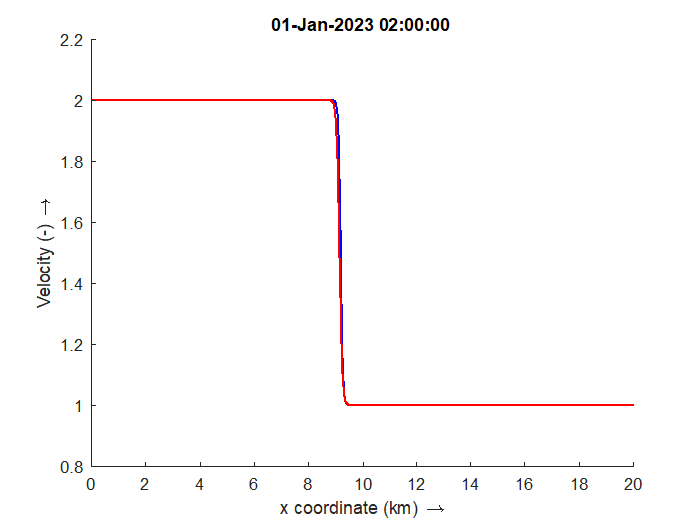
\includegraphics[width=\textwidth]{figures/nu020d0_velocity.png}
        \caption{Velocity along channel at $\bqty{2}{\hour}$.
        The blue line, without artificial viscosity and the red line with artificial velocity.
    }
    \end{subfigure}
    \hfill
    \begin{subfigure}{0.49\textwidth}
        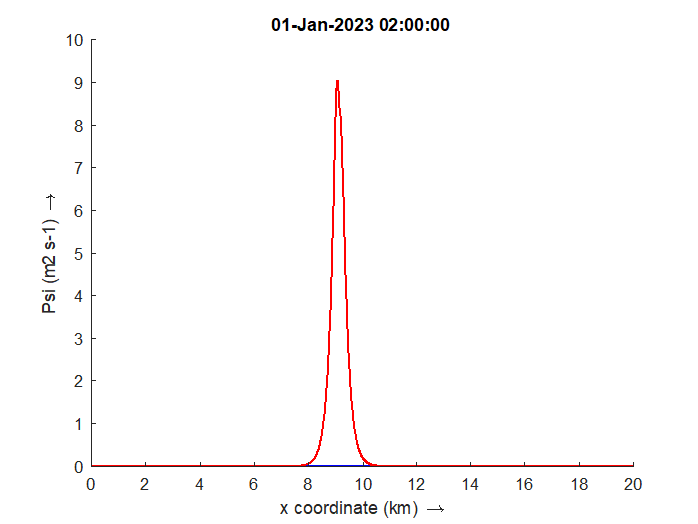
\includegraphics[width=\textwidth]{figures/nu020d0_psi.png}
        \caption{Used artificial viscoity $\Psi$ along channel at $\bqty{2}{\hour}$. The blue line, without artificial viscosity ($\equiv 0$) and the red line with artificial velocity.}
    \end{subfigure}
    \caption{Transect for velocity $\nu = \bqty{20}{\square\meter\per\second}$}
\end{figure}

\begin{figure}[H]
    \begin{subfigure}{0.49\textwidth}
        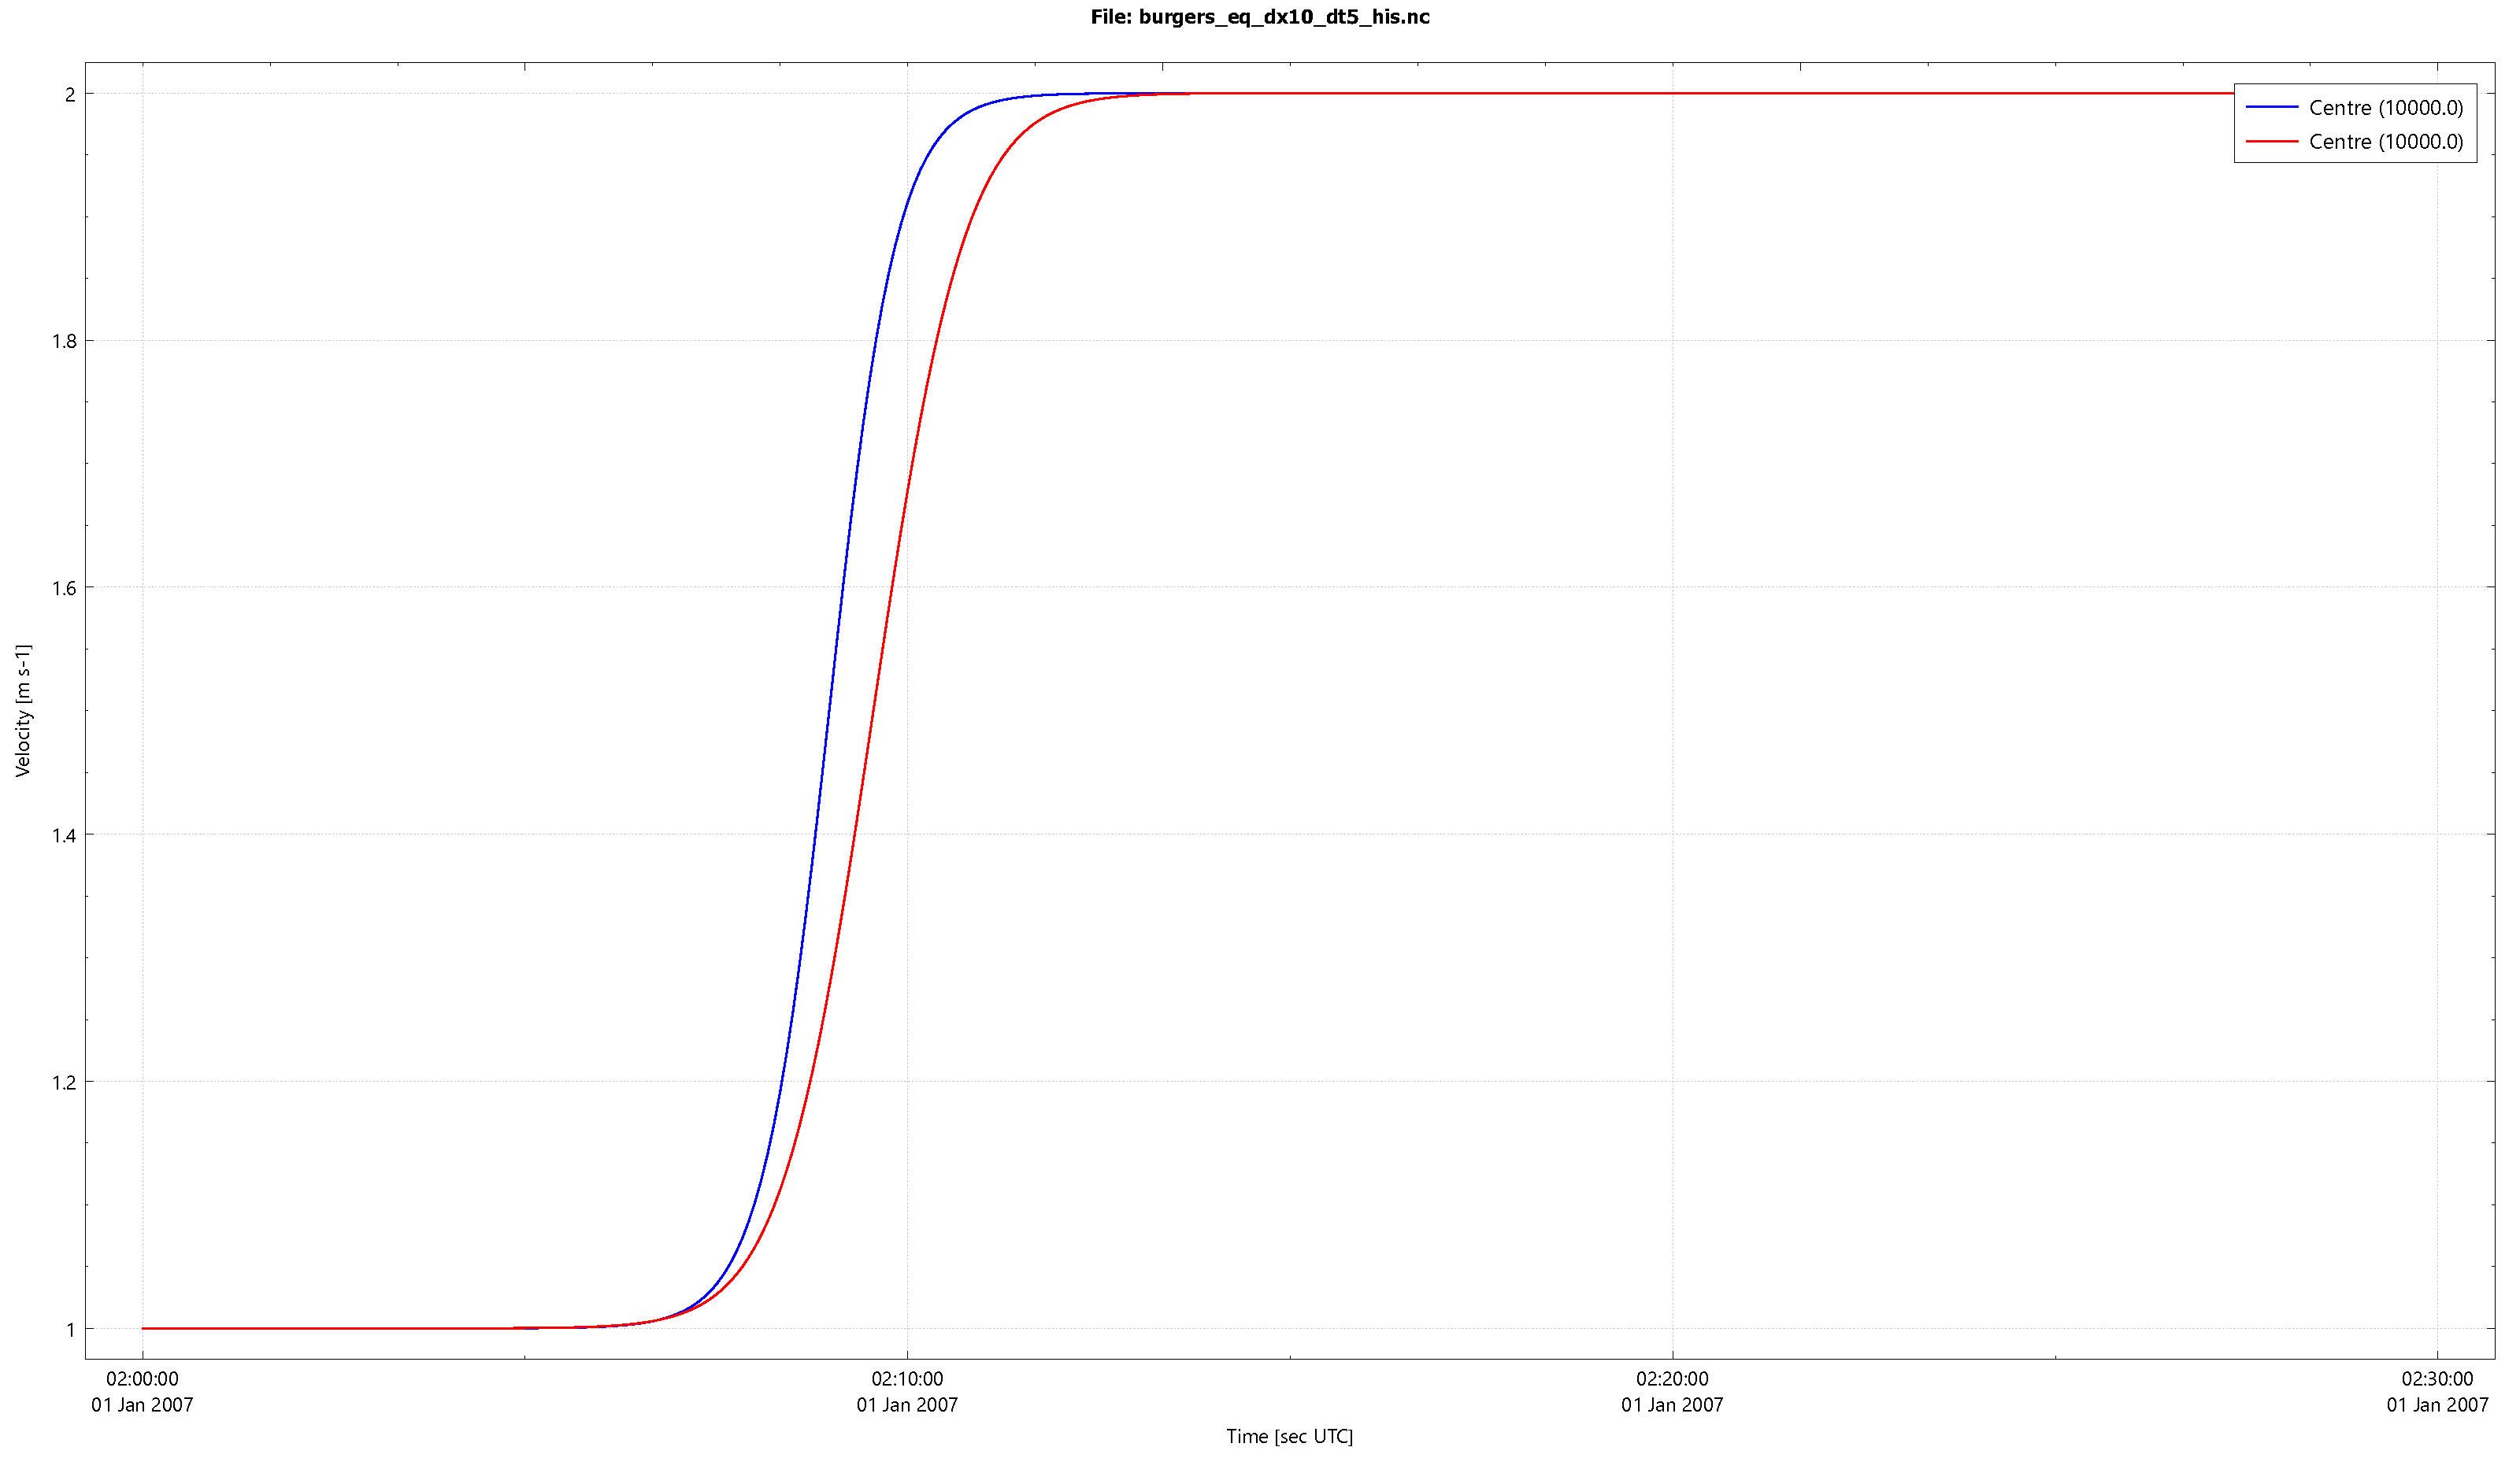
\includegraphics[width=\textwidth]{figures/20260603_115229.pdf}
        \caption{Time histories of the velocity for the observation point  at the centre of the channel. The blue line, without artificial viscosity and the red line with artificial velocity.}
    \end{subfigure}
    \hfill
    \begin{subfigure}{0.49\textwidth}
        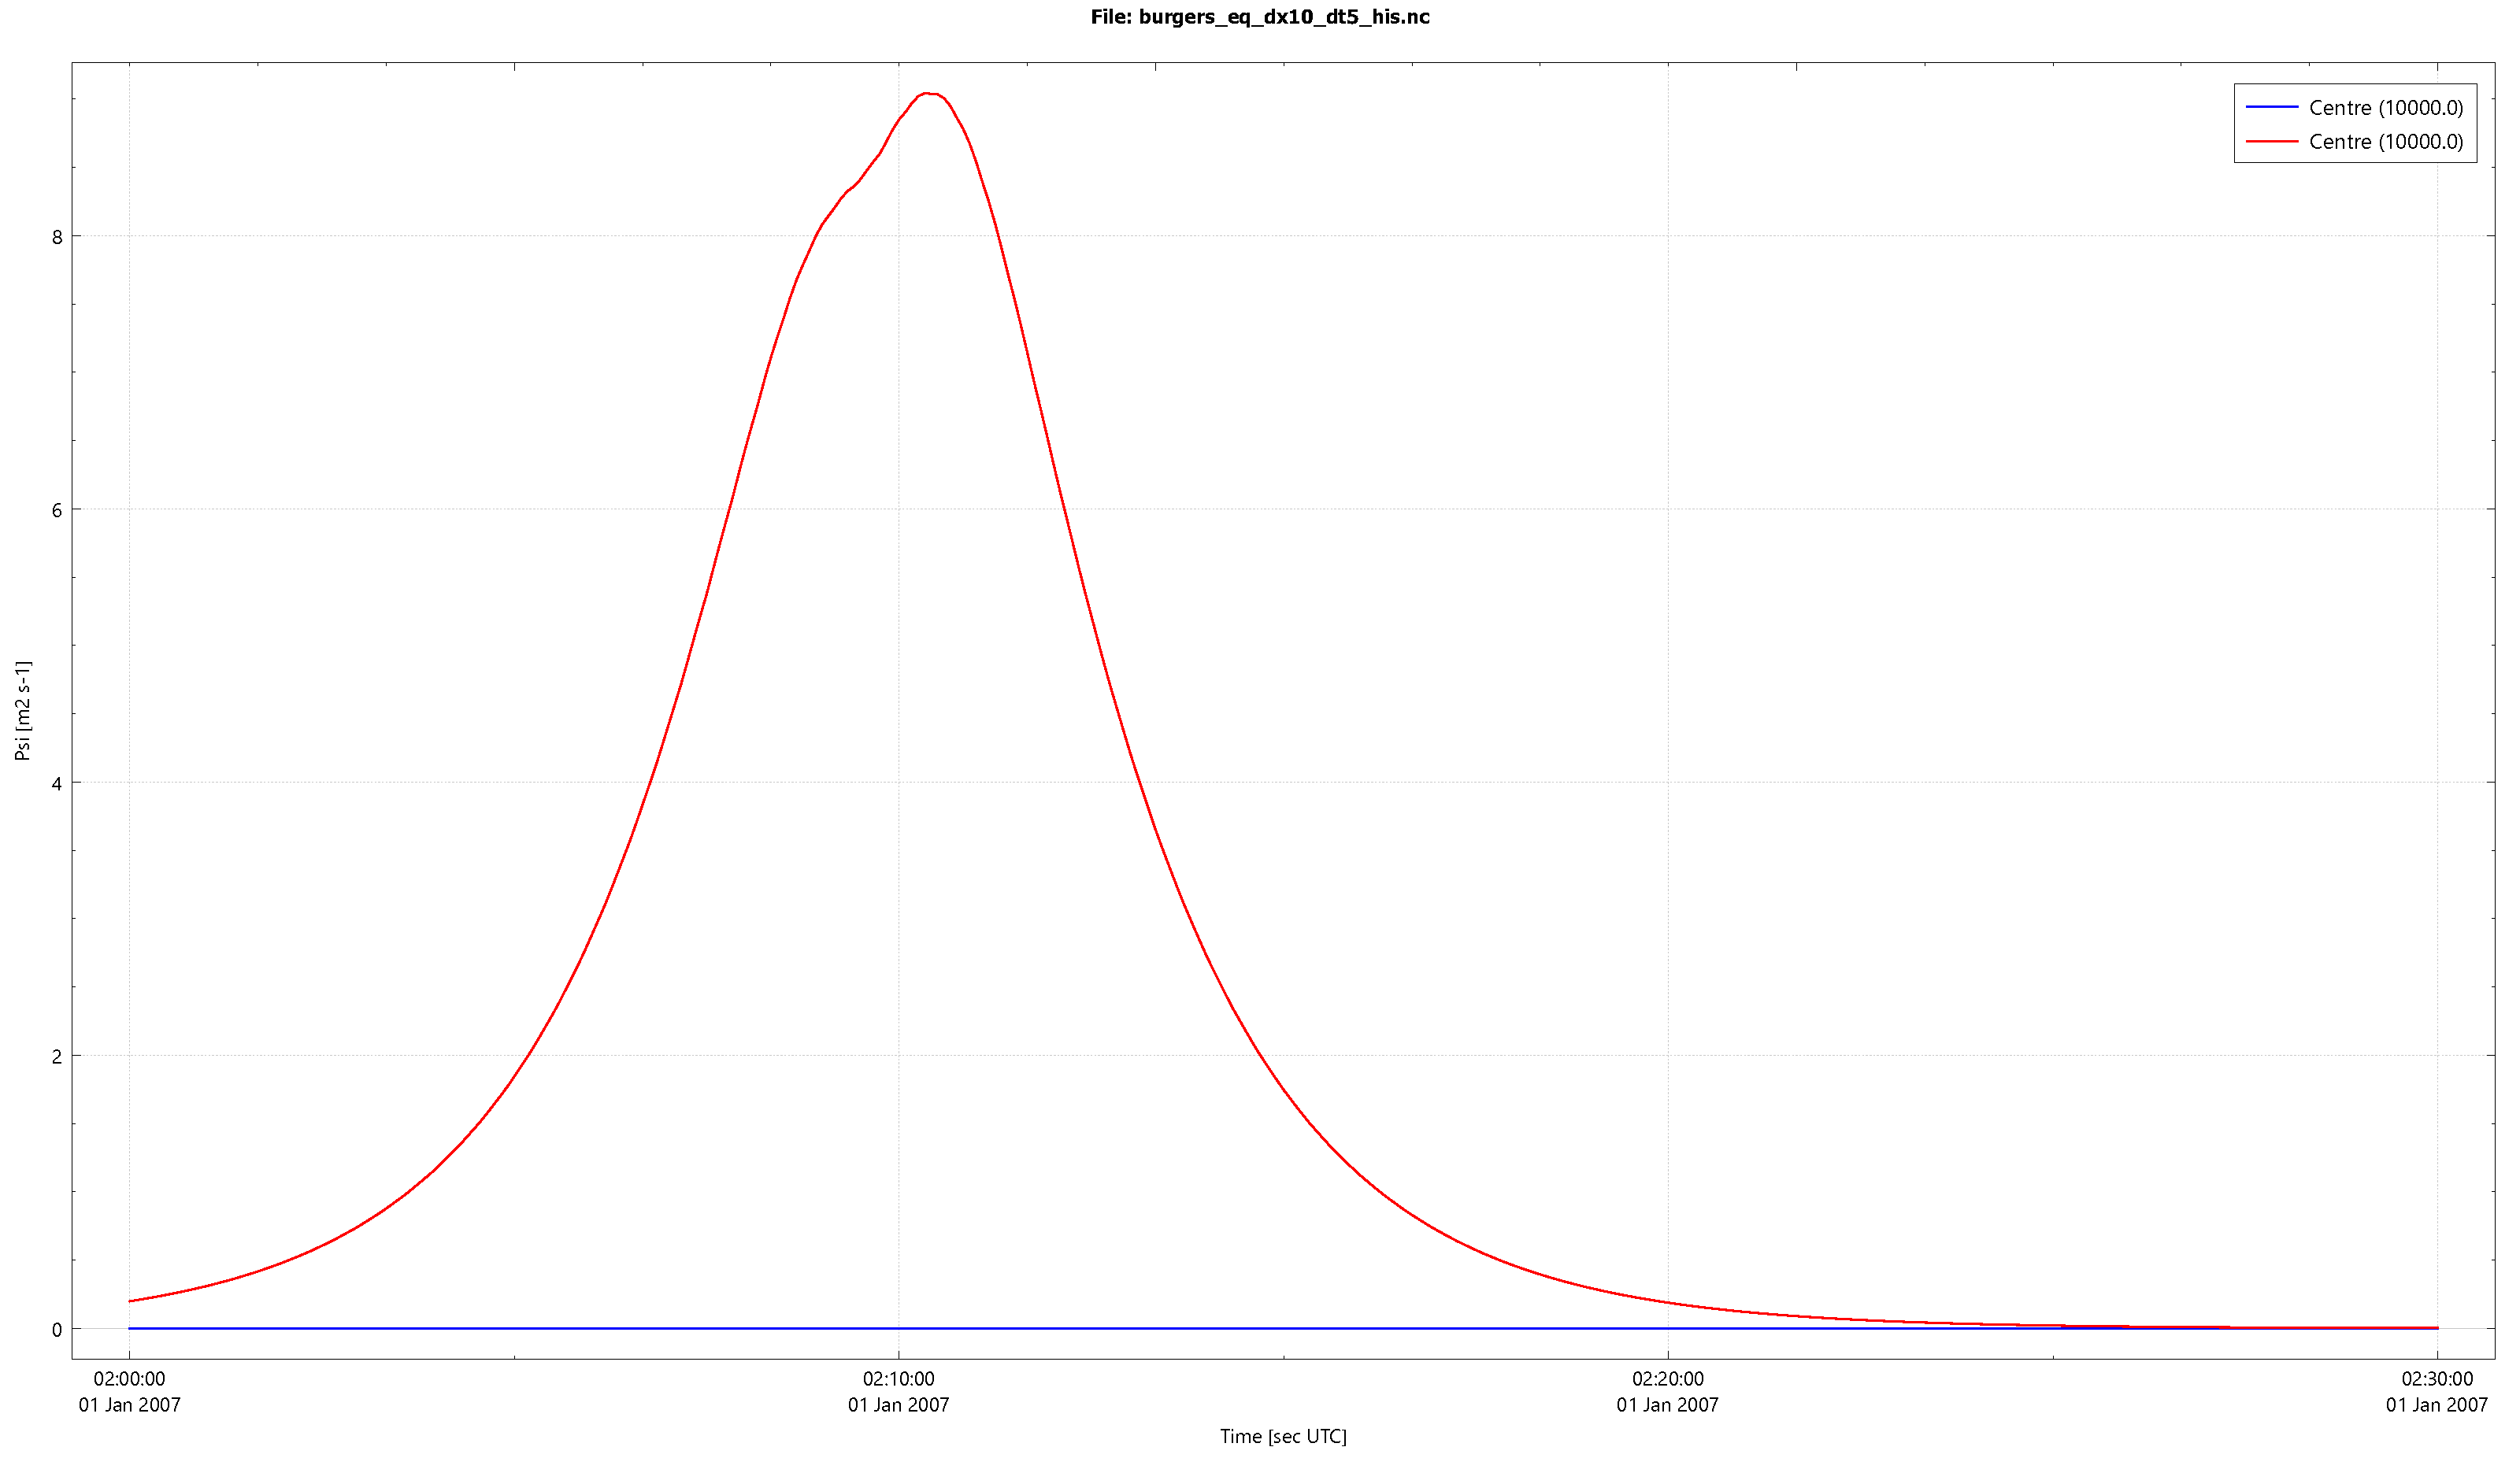
\includegraphics[width=\textwidth]{figures/20260603_115708.pdf}
                \caption{Time histories of the artificial viscosity $\Psi$ for the observation point at the $x=\bqty{10000}{\metre}$ (blue line) and at $x=\bqty{15000}{\metre}$ (red line).
                \newline \phantom{text}}
    \end{subfigure}
    \caption{Time histories for $\nu = \bqty{20}{\square\meter\per\second}$}
\end{figure}
\begin{figure}[H]
    \begin{subfigure}{0.8\textwidth}
        \centering
        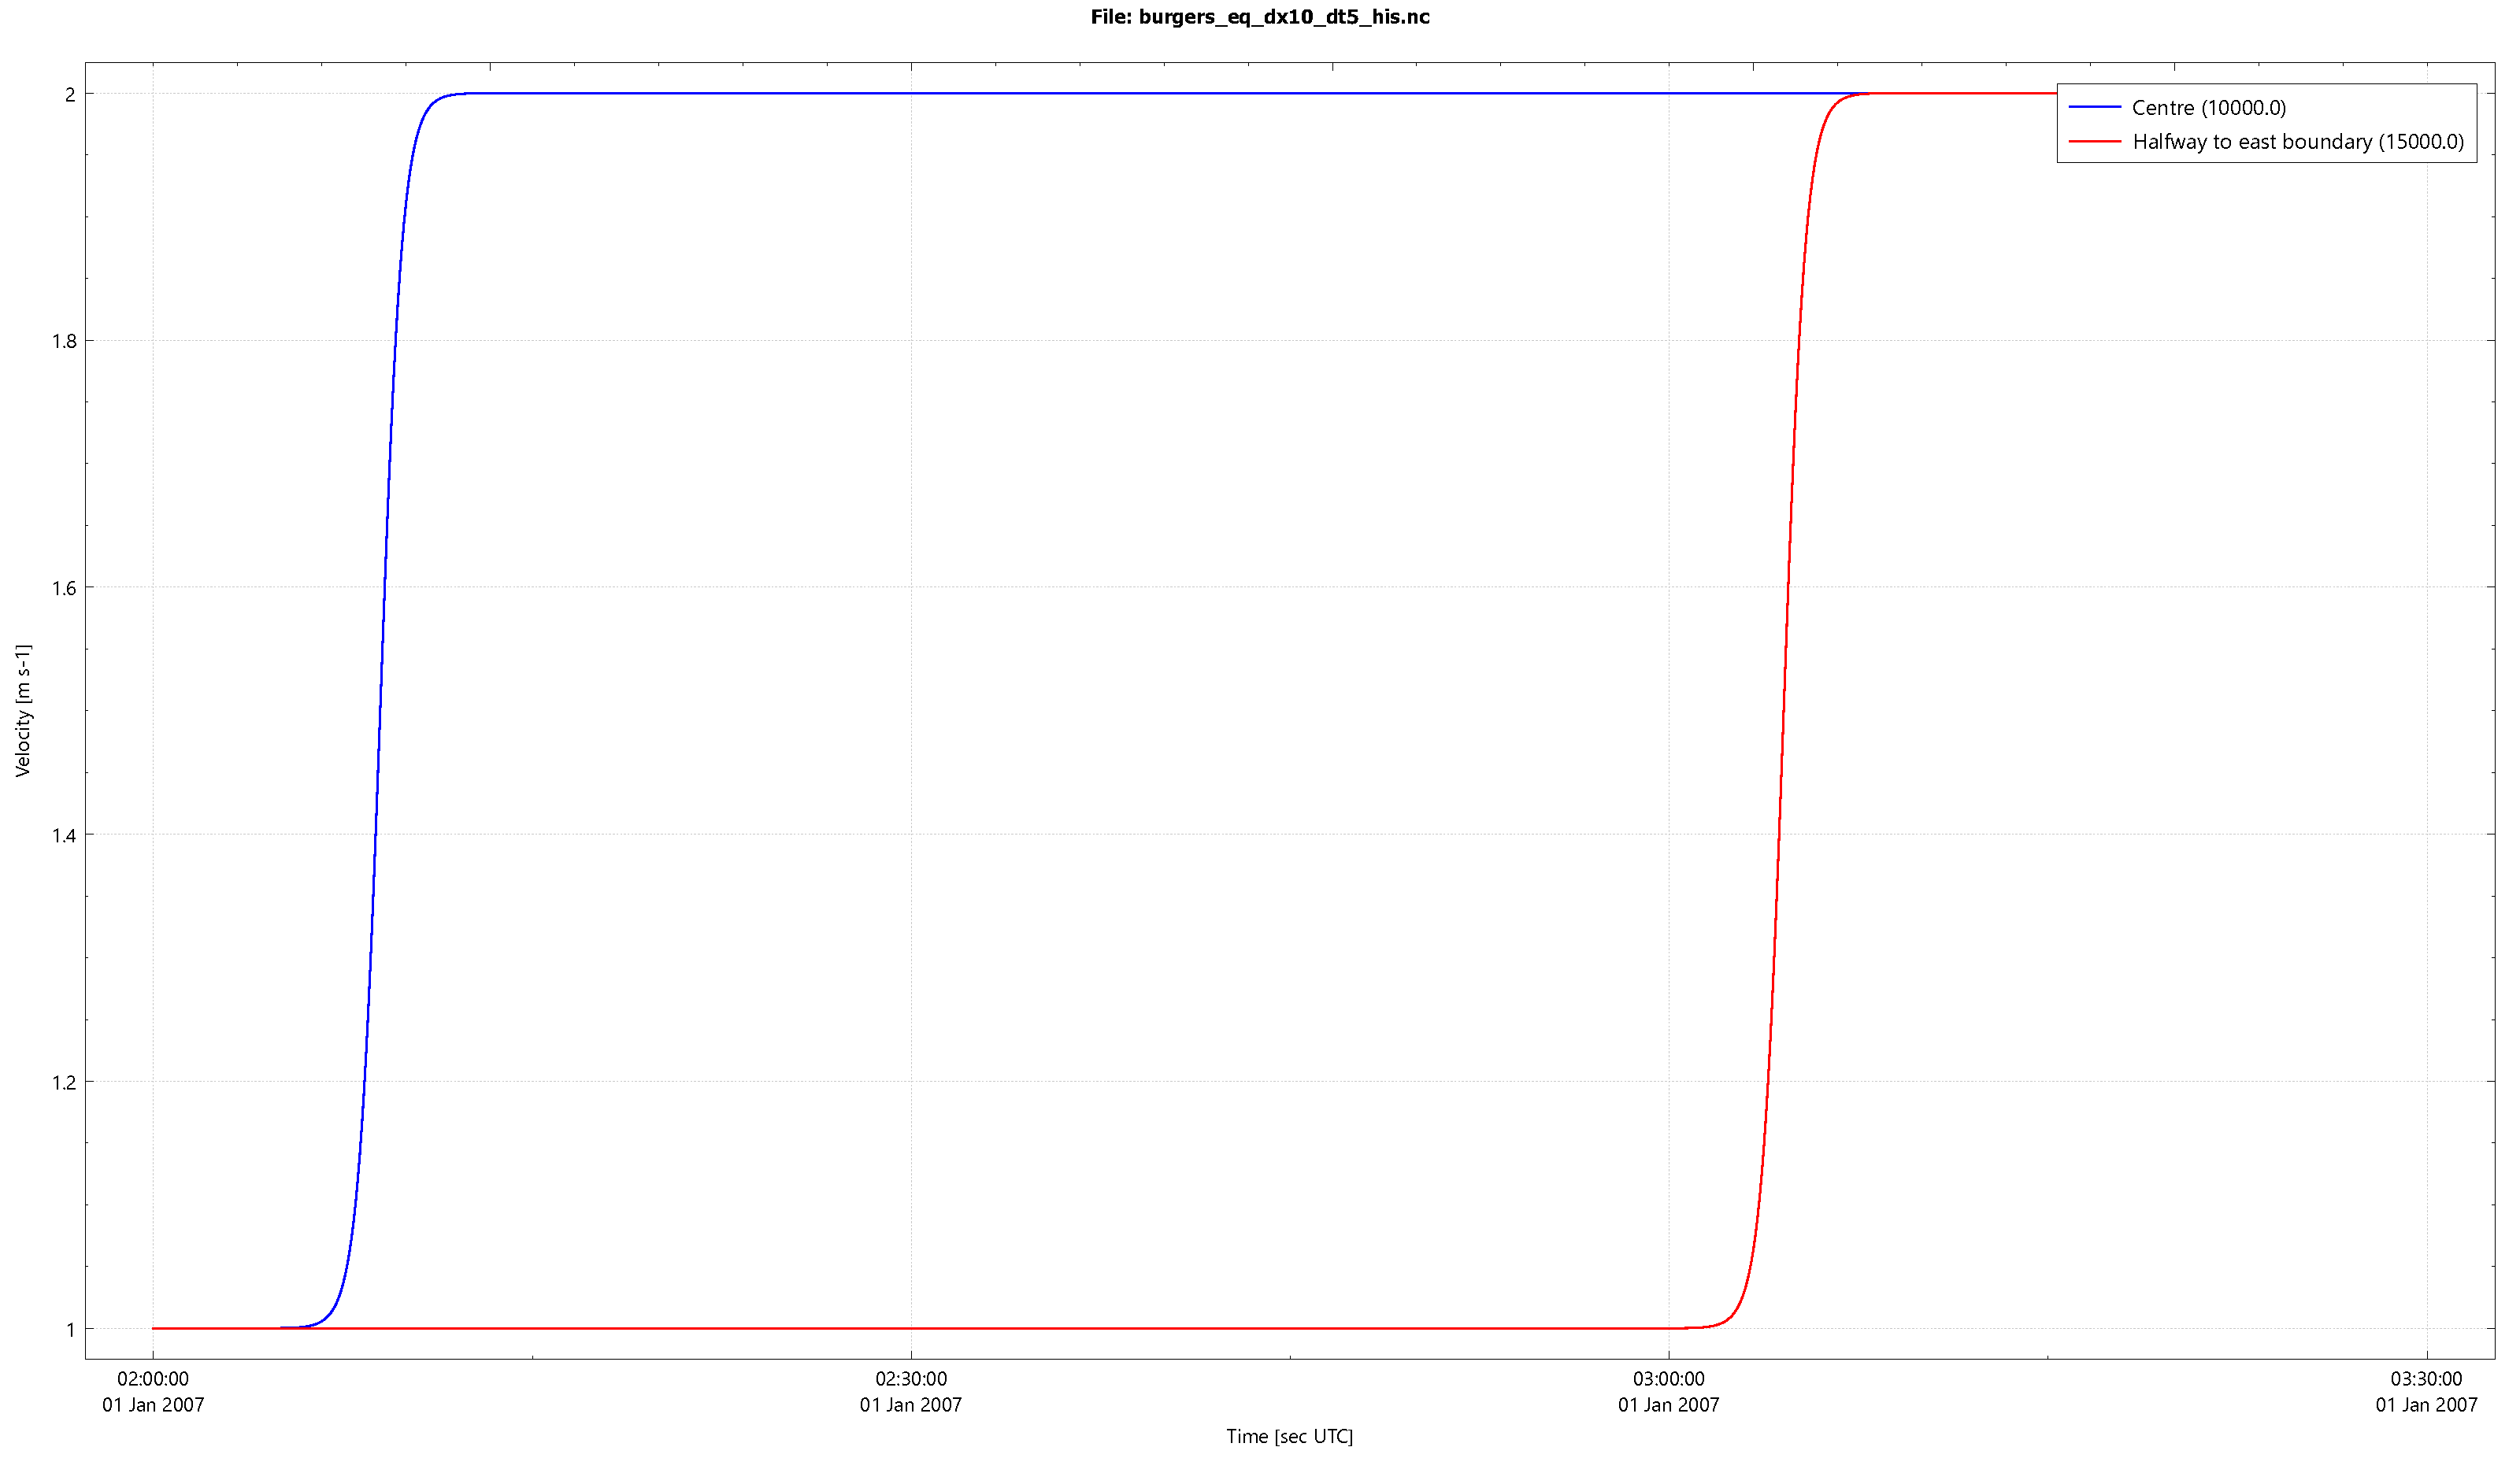
\includegraphics[width=\textwidth]{figures/vel_nu020d0_his_stat_hwaytoeast_centre.pdf}
        \caption{Time histories of the velocity for the observation point at the $x=\bqty{10000}{\metre}$ (blue line) and at $x=\bqty{15000}{\metre}$ (red line). \newline
            \phantom{text}}
    \end{subfigure}
    \begin{subfigure}{0.8\textwidth}
        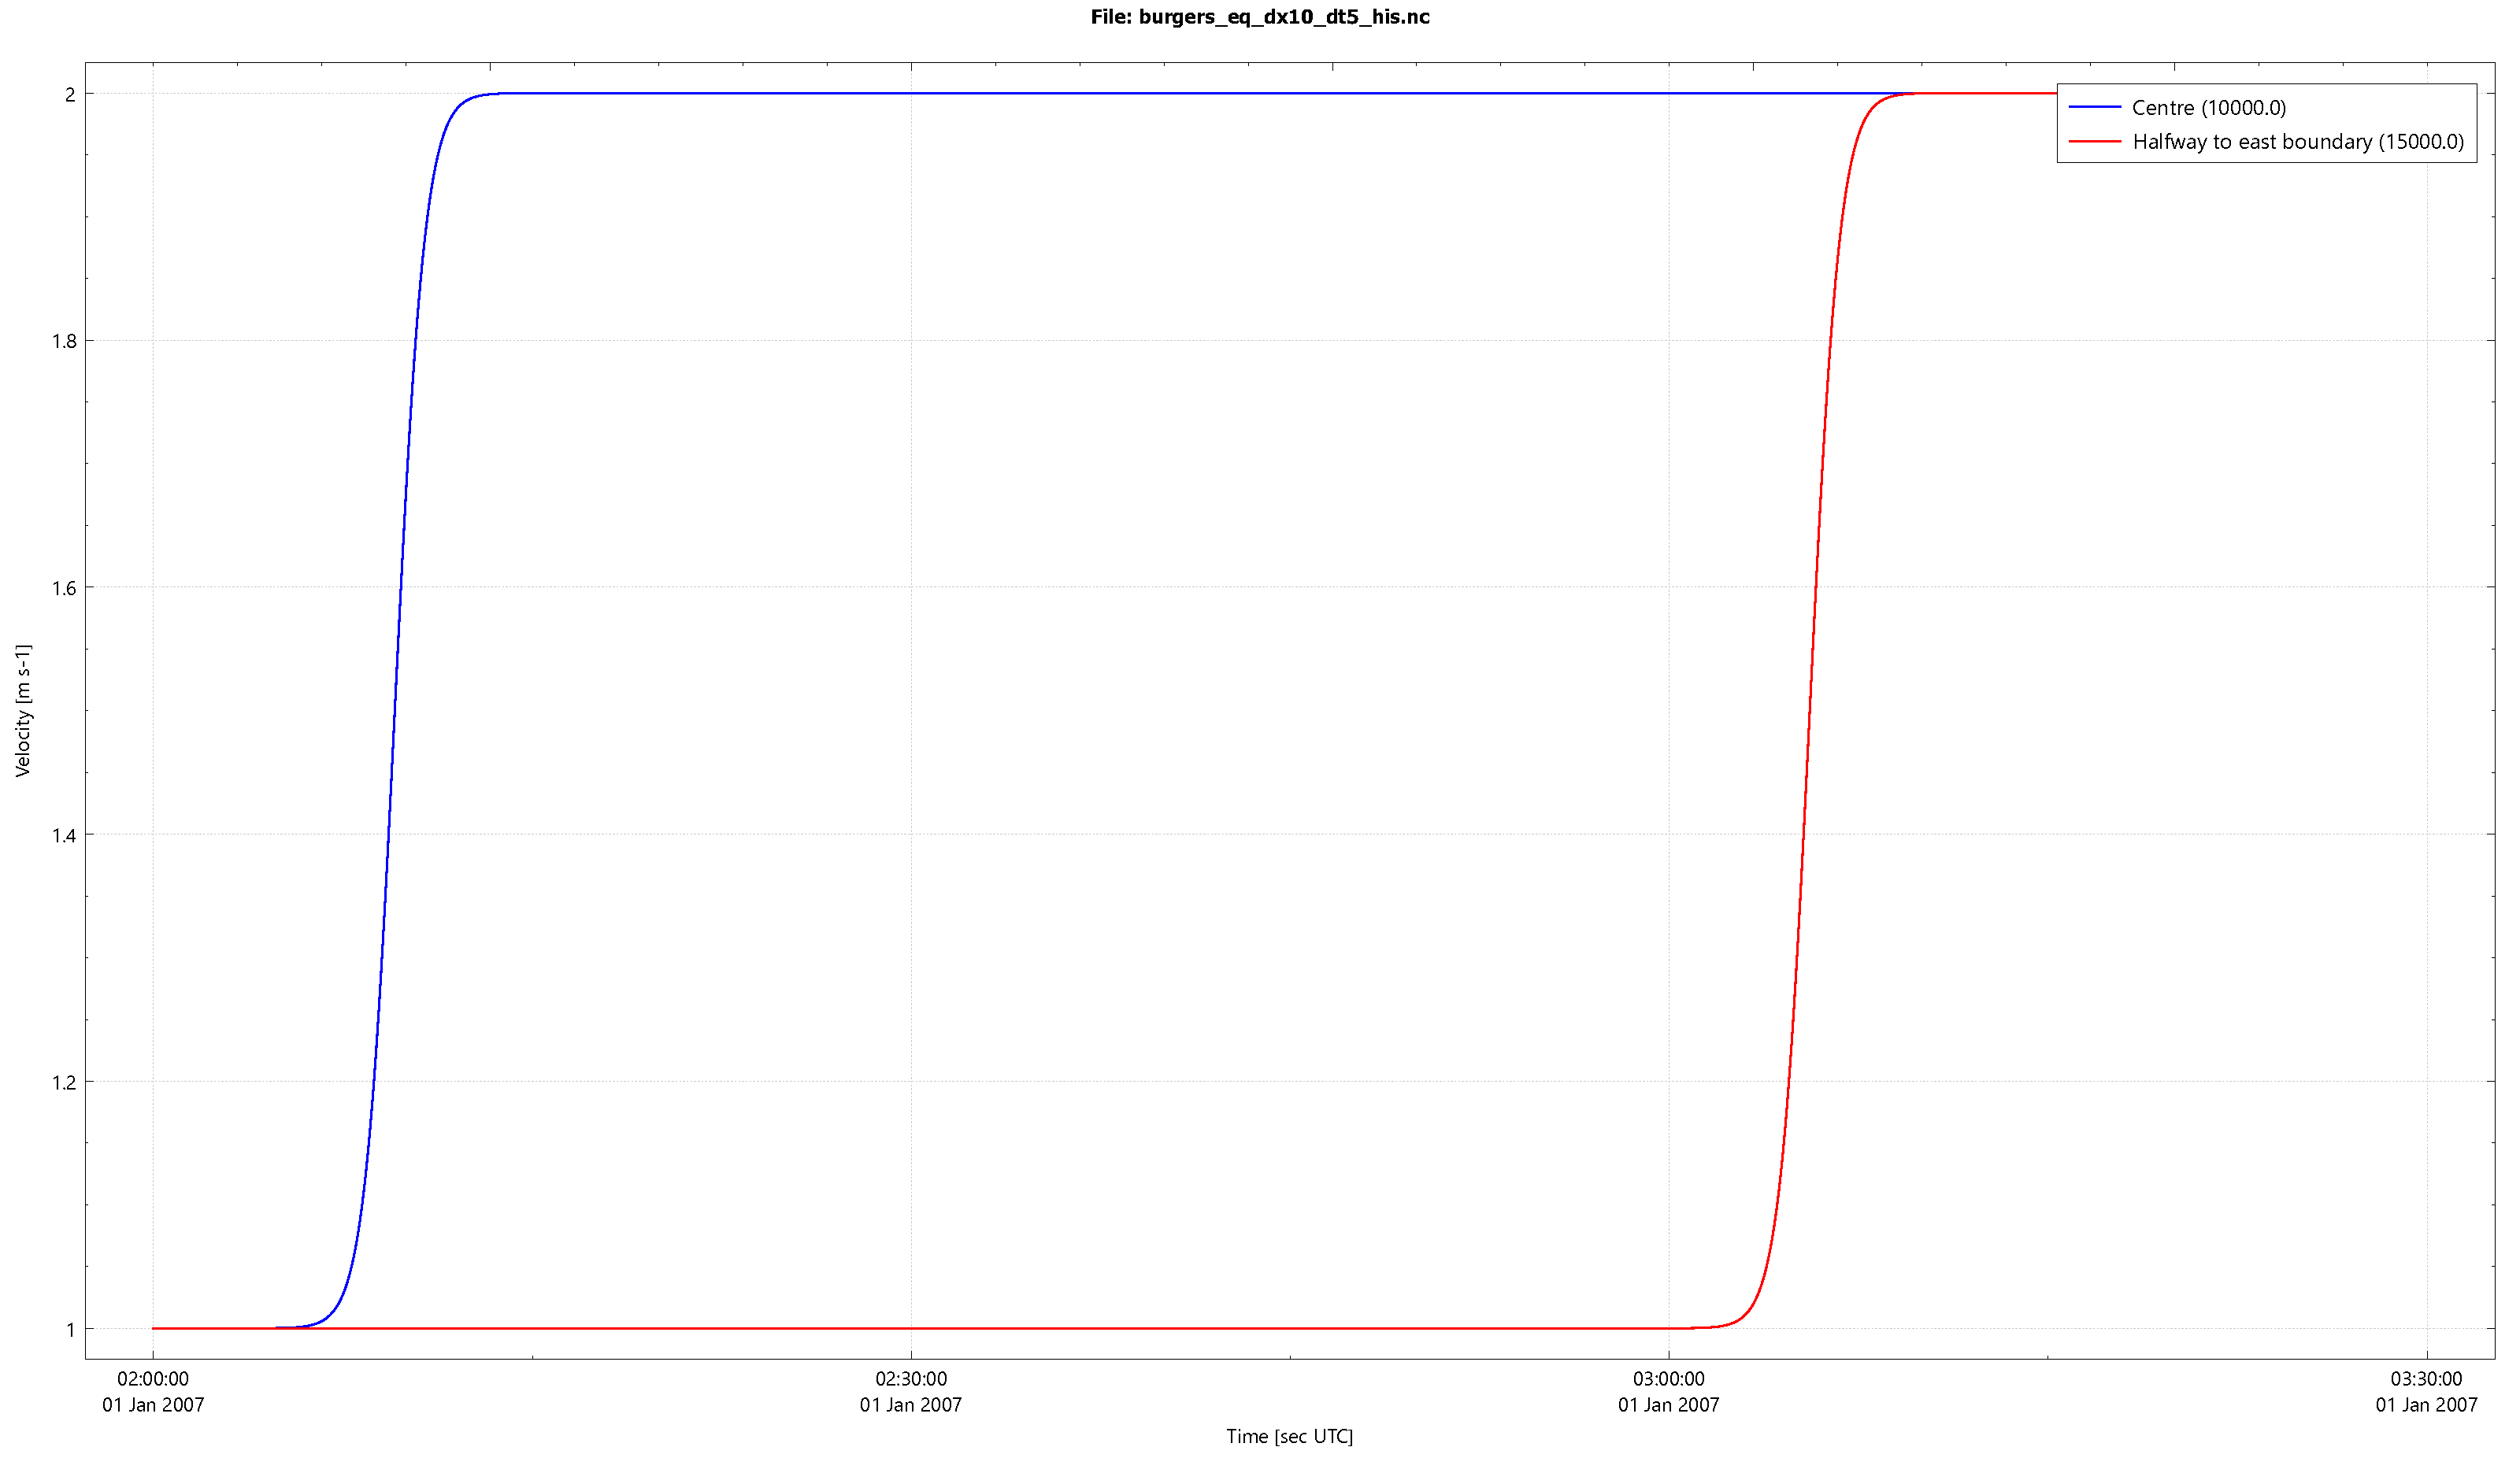
\includegraphics[width=\textwidth]{figures/vel_nu020d0_his_stat_hwaytoeast_centre_psi.pdf}
        \caption{Time histories of the artificial viscosity $\Psi$ for the observation point at the $x=\bqty{10000}{\metre}$ (blue line) and at $x=\bqty{15000}{\metre}$ (red line).}
    \end{subfigure}
    \caption{Time histories for when $\nu = \bqty{20}{\square\meter\per\second}$}
\end{figure}
The wave front has a speed of $u_{\it shock} = \bqty{1.5}{\metre\per\second}$ for both cases, without and with artificial viscosity (i.e. ${1.5000}$ vs $\bqty{1.4999}{\metre\per\second}$).
%----------------------------------------------------------
\section[Experiment with viscosity of 0.1 m2/s]{Experiment with viscosity of \bqty{0.1}{\metre\square\per\second}}
\begin{figure}[H]
    \begin{subfigure}{0.49\textwidth}
        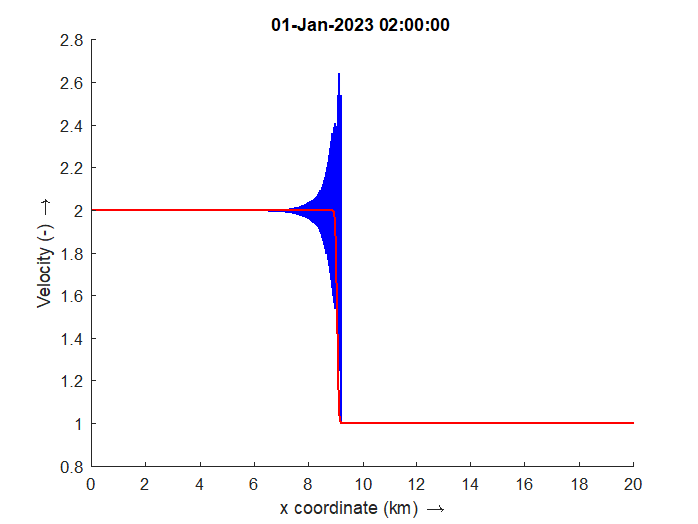
\includegraphics[width=\textwidth]{figures/nu000d1_velocity.png}
        \caption{Velocity along channel at $\bqty{2}{\hour}$. The blue line, without artificial viscosity and the red line with artificial velocity.
        }
    \end{subfigure}
    \hfill
    \begin{subfigure}{0.49\textwidth}
        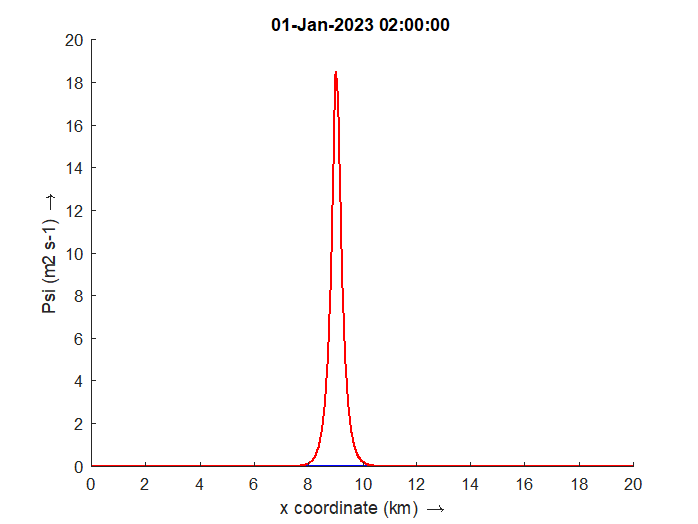
\includegraphics[width=\textwidth]{figures/nu000d1_psi.png}
        \caption{Used artificial viscoity $\Psi$ along channel at $\bqty{2}{\hour}$. The blue line, without artificial viscosity ($\equiv 0$) and the red line with artificial velocity.}
    \end{subfigure}
    \caption{Transect for velocity $\nu = \bqty{0.1}{\square\meter\per\second}$}
\end{figure}

\begin{figure}[H]
    \begin{subfigure}{0.49\textwidth}
        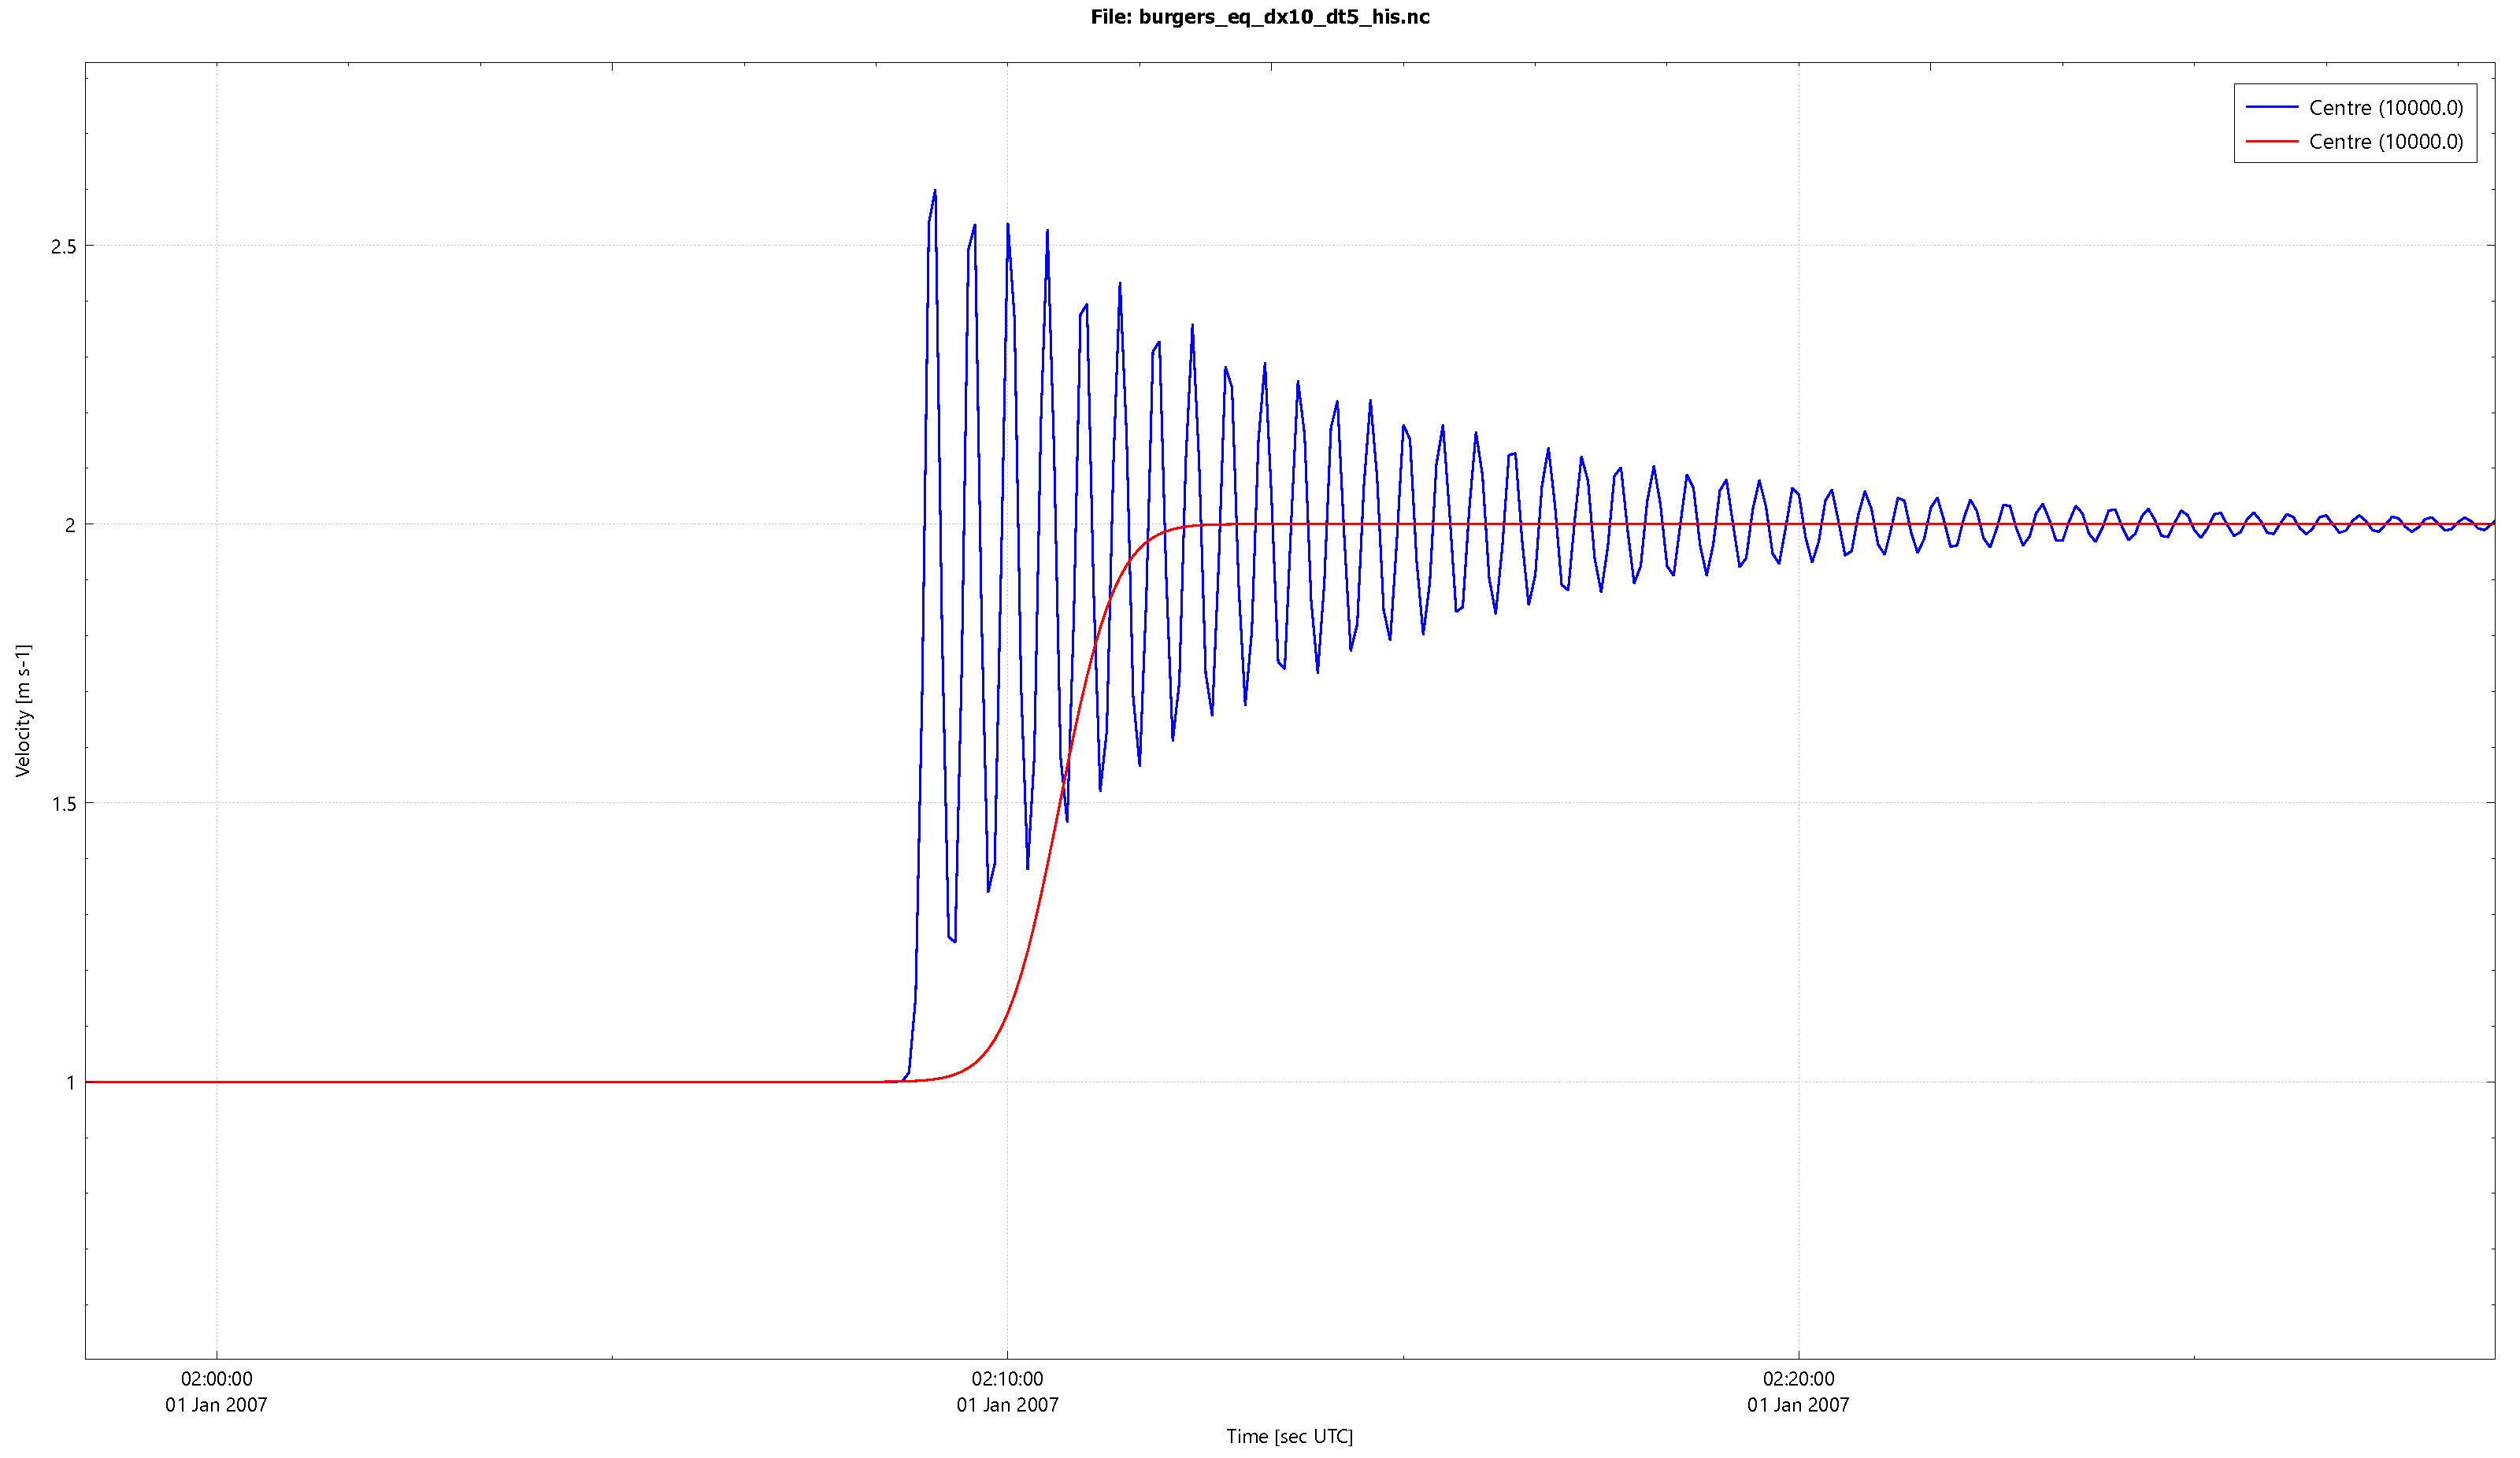
\includegraphics[width=\textwidth]{figures/20260602_224544.pdf}
        \caption{Time histories of the velocity for the observation point  at the centre of the channel. The blue line, without artificial viscosity and the red line with artificial velocity. \newline
        \phantom{text}}
    \end{subfigure}
    \hfill
    \begin{subfigure}{0.49\textwidth}
        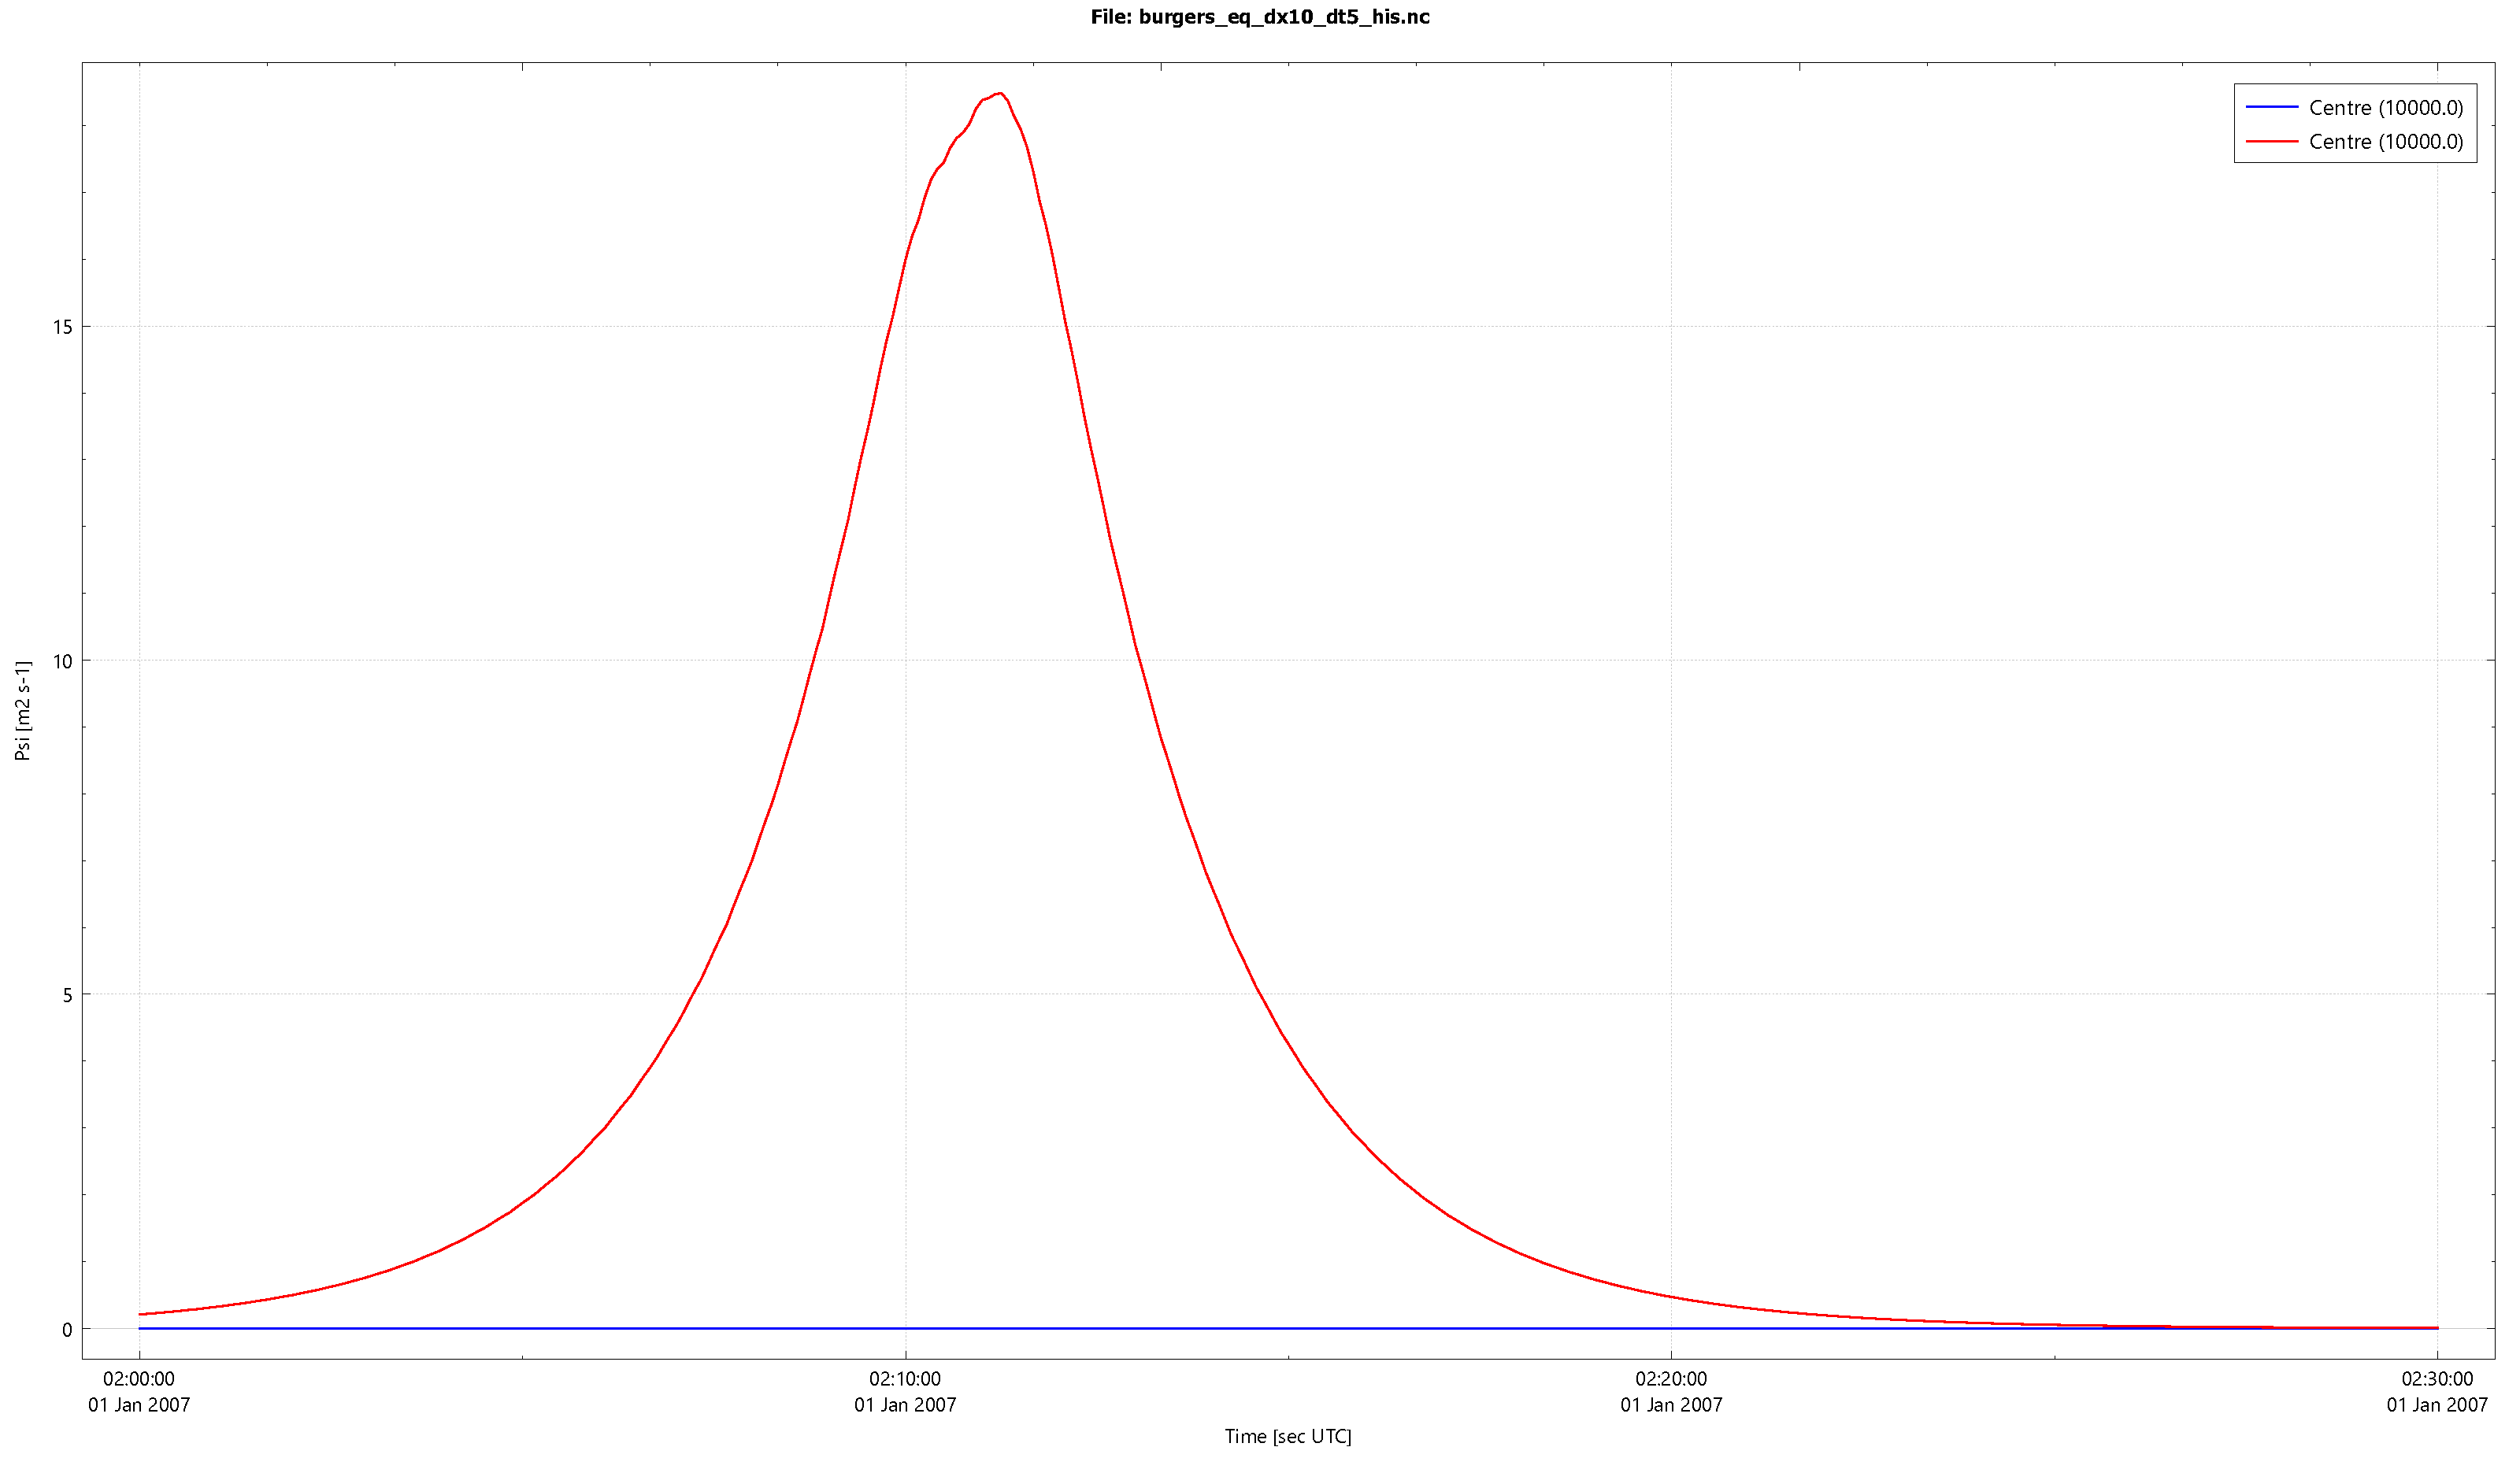
\includegraphics[width=\textwidth]{figures/20260602_225828.pdf}
        \caption{Time histories of the artificial viscosity $\Psi$ for the observation point  at the centre of the channel. The blue line, without artificial viscosity ($\equiv 0$) and the red line with artificial velocity.}
    \end{subfigure}
    \caption{Time histories for $\nu = \bqty{0.1}{\square\meter\per\second}$}
\end{figure}
\begin{figure}[H]
    \begin{subfigure}{0.8\textwidth}
        \centering
        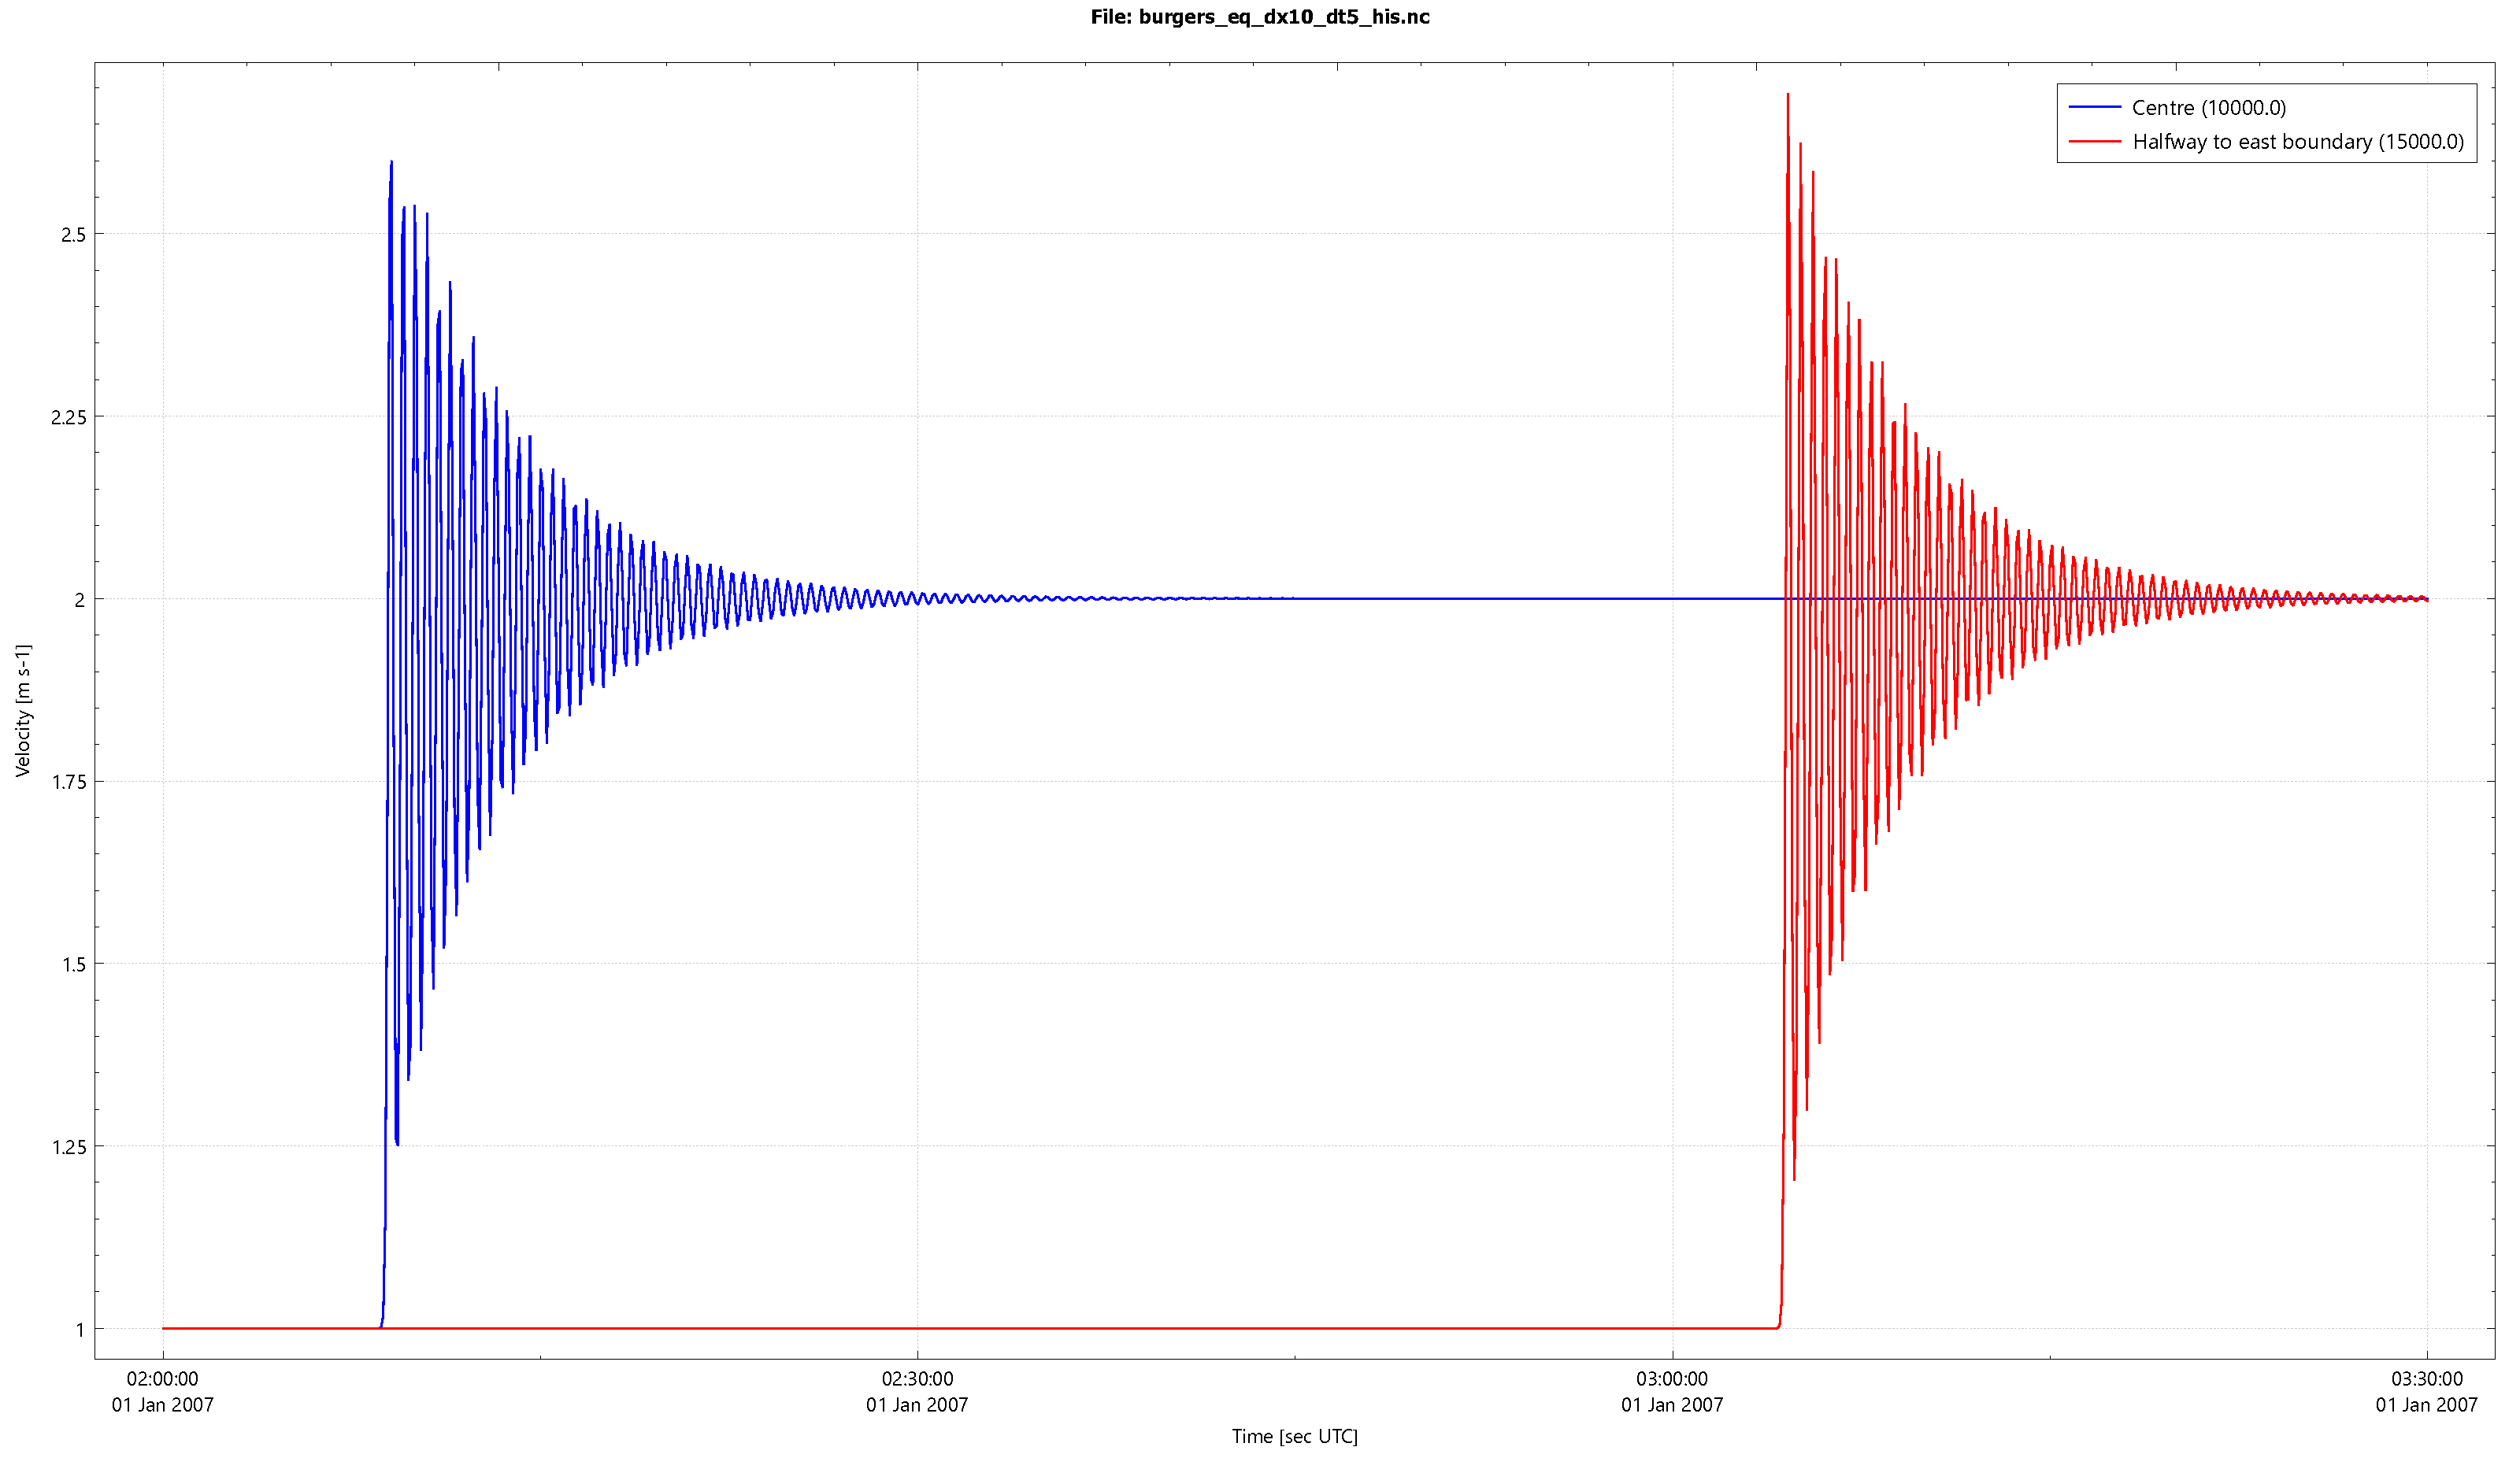
\includegraphics[width=\textwidth]{figures/vel_nu000d1_his_stat_hwaytoeast_centre.pdf}
        \caption{Time histories of the velocity for the observation point at the $x=\bqty{10000}{\metre}$ (blue line) and at $x=\bqty{15000}{\metre}$ (red line). \newline
            \phantom{text}}
    \end{subfigure}
    \begin{subfigure}{0.8\textwidth}
        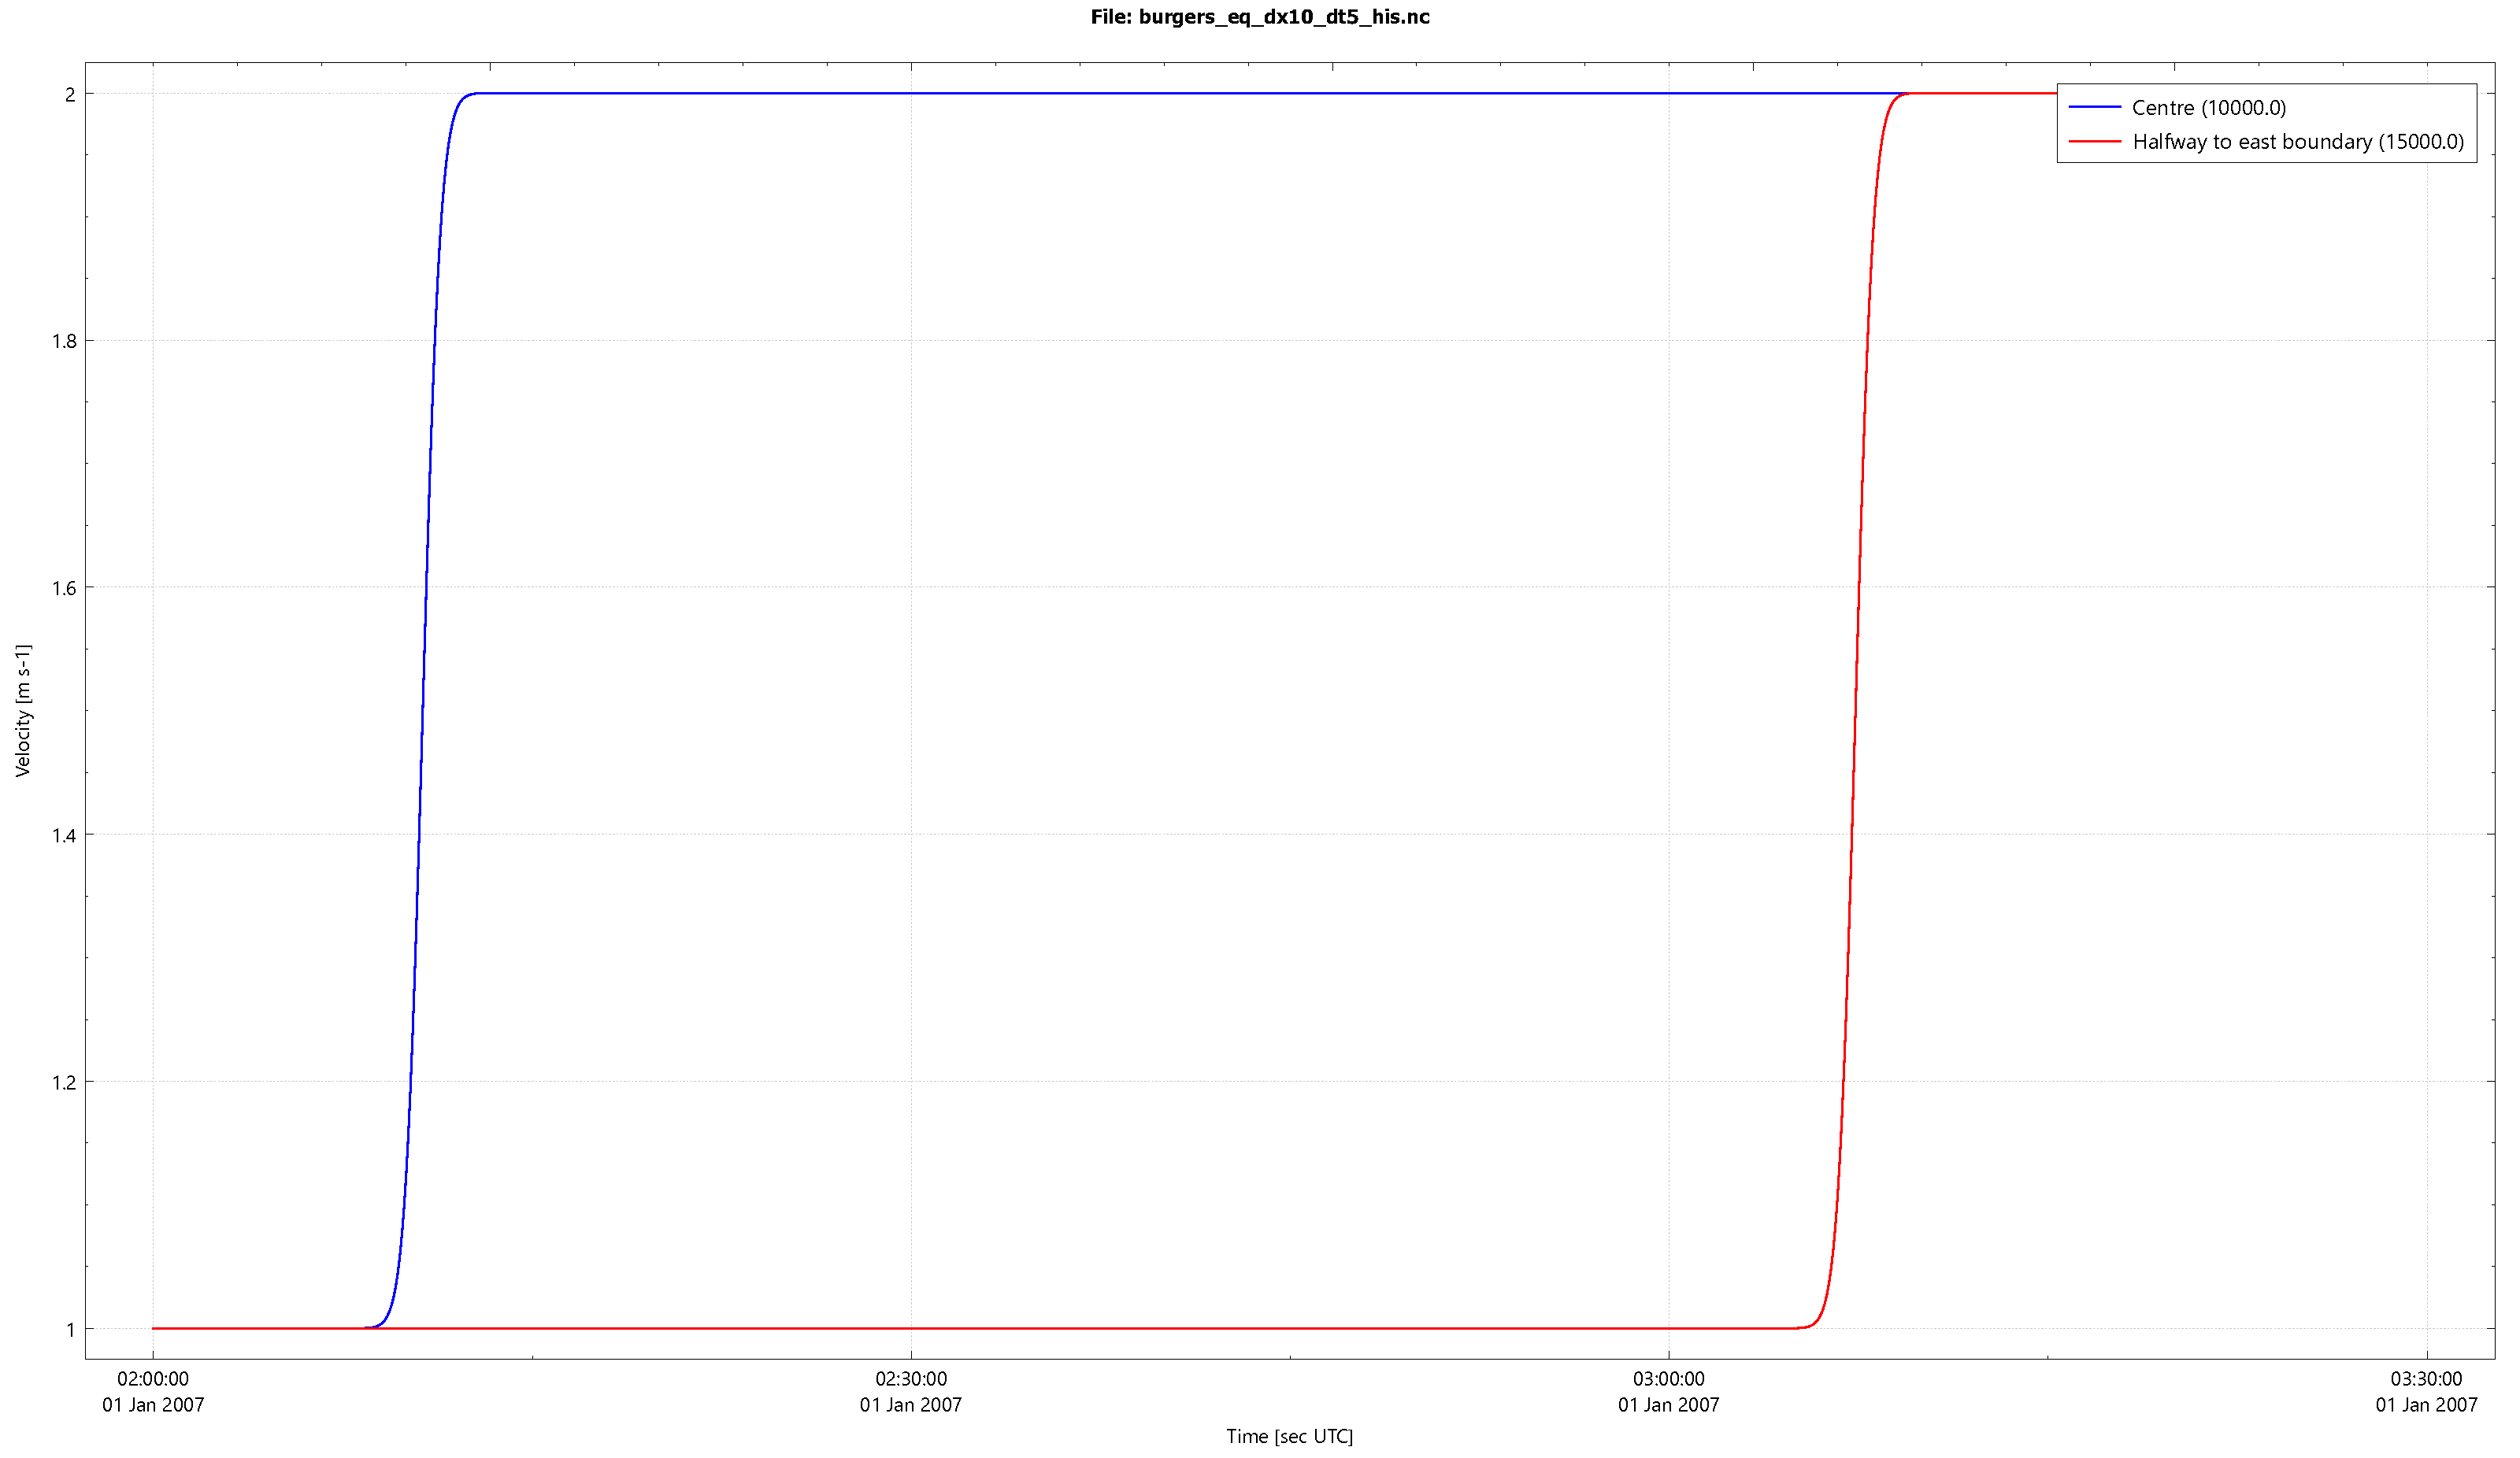
\includegraphics[width=\textwidth]{figures/vel_nu000d1_his_stat_hwaytoeast_centre_psi.pdf}
                \caption{Time histories of the artificial viscosity $\Psi$ for the observation point at the $x=\bqty{10000}{\metre}$ (blue line) and at $x=\bqty{15000}{\metre}$ (red line).}
    \end{subfigure}
    \caption{Time histories for when $\nu = \bqty{0.1}{\square\meter\per\second}$}
\end{figure}
The wave front has a speed of $u_{\it shock} = \bqty{1.5}{\metre\per\second}$ for both cases, without and with artificial viscosity (i.e. ${1.5000}$ vs $\bqty{1.5000}{\metre\per\second}$).

%-------------------------------------------------------------------------------
%\subsection{Constant viscosity $\nu$}
%-------------------------------------------------------------------------------
\section{Experiment with non linear source term}
This experiment is taken from \citet{Colombo2026} and read
\begin{align}
    \pdiff{u}{t} + u \pdiff{u}{x} - \nu \pdiff[2]{u}{x}= u^2, \quad u >0
\end{align}
With viscosity coefficient $\nu = \bqty{0.0}{\square\metre\per\second}$ and initial condition
\begin{align}
u(x,0) = \exp(x) + 0.3 \exp( -200 (x + 0.5)^2), \quad x\in = [-1,1]
\end{align}
and boundary condition at the left side
\begin{align}
    u(-1,t) = \exp(-1).
\end{align}


\notyet
\printallbibliography
\appendix
%\chapter{Taylor Series of \( \frac{1}{3} u(x)^3 \) about \( x = 0 \)}
\section{Taylor Series of \( \frac{1}{3} u(x)^3 \) about \( x = 0 \)}
Let \( f(x) = \frac{1}{3} u(x)^3 \), where \( u = u(x) \).
The Taylor series about \( x = 0 \) is given by:
%
\begin{align}
    f(x) = f(0) + f'(0) x + \frac{f''(0)}{2!} x^2 + \frac{f'''(0)}{3!} x^3 + \cdots
\end{align}
%
\subsection*{Step 1: Compute derivatives}
\begin{align}
    \begin{aligned}
        f(x) &= \frac{1}{3} u^3, \\
        f'(x) &= u^2 u', \\
        f''(x) &= 2 u (u')^2 + u^2 u'', \\
        f'''(x) &= 2 (u')^3 + 6 u u' u'' + u^2 u''',
    \end{aligned}
\end{align}
%
where \( u' = \frac{du}{dx}, u'' = \frac{d^2 u}{dx^2}, u''' = \frac{d^3 u}{dx^3} \).
%
\subsection*{Step 2: Substitute \( x = 0 \) into derivatives}
\begin{align}
    \begin{aligned}
        f(0) &= \frac{1}{3} u(0)^3, \\
        f'(0) &= u(0)^2 u'(0), \\
        f''(0) &= 2 u(0) (u'(0))^2 + u(0)^2 u''(0), \\
        f'''(0) &= 2 (u'(0))^3 + 6 u(0) u'(0) u''(0) + u(0)^2 u'''(0)
    \end{aligned}
\end{align}
%
\subsection*{Step 3: Taylor series expansion}
\begin{align}
    \frac{1}{3} u(x)^3 &= \frac{1}{3} u(0)^3
    + u(0)^2 u'(0) x
    + \Big( u(0) (u'(0))^2 + \frac{1}{2} u(0)^2 u''(0) \Big) x^2 +
    \\
    & + \Big( \frac{1}{3} (u'(0))^3 + u(0) u'(0) u''(0) + \frac{1}{6} u(0)^2 u'''(0) \Big) x^3 + \cdots
\end{align}

%------------------------------------------------------------------------------
\end{document}
